
\documentclass[11pt]{article}


%  sudo apt-get install culmus
%  sudo apt-get install texlive-xetex
%  sudo apt-get install texlive-latex-extra
%  sudo apt-get install texlive-lang-hebrew
%  sudo apt-get install texlive-lang-other texlive-lang-arabic
%  sudo apt-get install texlive-fonts-extra texlive-latex-extra


\makeatletter
\def\Year#1{%
  \def\yy@##1##2##3##4;{##1##2##3##4}%
  \expandafter\yy@#1;
}
\makeatother


\usepackage[utf8]{inputenc}
\usepackage{titlesec}
\usepackage{lipsum}
\usepackage{listings}
\lstset{
  columns=fullflexible,
  frame=single,
  breaklines=true
}

\setcounter{secnumdepth}{4}
\titleformat{\paragraph}
{\normalfont\normalsize\bfseries}{\theparagraph}{1em}{}
\titlespacing*{\paragraph}
{0pt}{3.25ex plus 1ex minus .2ex}{1.5ex plus .2ex}

\usepackage{graphicx}
\graphicspath{ {images/} }


\makeatother
\usepackage[hyphens]{url}

\usepackage{polyglossia}
\setdefaultlanguage{english}
\setotherlanguage{hebrew}
\setotherlanguage[variant=ancient]{greek}
\usepackage{fontspec}
\newfontfamily\greekfont[Script=Greek]{Linux Libertine O}


%linux settings
\setmonofont{Miriam Mono CLM}
\setsansfont{Simple CLM}
\setmainfont{Frank Ruehl CLM}


%windows settings
%\setmainfont{Arial}
% to change font for Hebrew
%\newfontfamily\hebrewfonttt[Script=Hebrew]{Miriam Mono CLM}
%\newfontfamily\hebrewfontsf[Script=Hebrew]{Simple CLM}
%\newfontfamily\hebrewfont[Script=Hebrew]{David CLM}

\usepackage{datetime2}

\usepackage[backend=biber]{biblatex}
\bibliography{\jobname}
\begin{filecontents}{\jobname.bib}
  @book{lit1,
    author      =   {Author, A. N.},
    title       =   {Title},
    publisher   =   {Publisher},
    address     =   {Location},
    year        =   {1066}}
\end{filecontents}

%makeatletter

\DeclareCiteCommand{\textcite}
  {\iffootnote{\usebibmacro{cite:init}}{}%
   \usebibmacro{prenote}}%
  {\usebibmacro{citeindex}%
   \iffootnote
     {\global\booltrue{cbx@mlafootnotes}%
      \renewcommand*{\newunitpunct}{\addcomma\space}%
      \usebibmacro{cite:mla:foot}}
     {\usebibmacro{cite:mla}}}
  {}
  {\usebibmacro{mla:foot:postnote}}

\makeatother

%\bibliography{biblatex-examples}

\newcommand{\cmd}[1]{\texttt{\textbackslash #1}}
\setlength{\parindent}{0pt}




\title{\textbf{An Argument for Biblical Ethics} \large \\ problem verses and controversy (rough draft) }
\begin{large}

\end{large}
\author{\textcircled{c} 2018-\the\year
 \ Anonymous \\ GNU Free Documentation License  }
\date{created: 2018--09 -20 \\ last updated: \today{}}
\begin{document}

\maketitle
\tableofcontents 

\noindent \newline Copyright (C) 2018-\the\year
 \ Anonymous \ GNU Free Documentation License \newline
Permission is granted to copy, distribute and/or modify this document\newline
under the terms of the GNU Free Documentation License, Version 1.3\newline
or any later version published by the Free Software Foundation;\newline
with no Invariant Sections, no Front-Cover Texts, and no Back-Cover Texts.\newline
A copy of the license is included in the section entitled "GNU\newline
Free Documentation License" at the end of this document.

\section{Introduction}
To begin with a disclaimer I am not arguing that we setup a community that practices Biblical law in any country that won't tolerate it. To set up a legal system against one country while inside of it is an act of war or rebellion. The Tanahk does not give us authority to do this and in fact I believe 1 Peter 2:13-17 precludes this for governments that in general uphold what is good and punish evil: 

\begin{quote}
1 Peter 2:13-17 Young's Literal Translation (YLT)
13 Be subject, then, to every human creation, because of the Lord, whether to a king, as the highest,
14 whether to governors, as to those sent through him, for punishment, indeed, of evil-doers, and a praise of those doing good;
15 because, so is the will of God, doing good, to put to silence the ignorance of the foolish men;
16 as free, and not having the freedom as the cloak of the evil, but as servants of God;
17 to all give ye honour; the brotherhood love ye; God fear ye; the king honour ye.
\end{quote}

It should be taken into consideration that even the Roman empire which practiced many barbarous things was an empire that upheld order. When the Roman empire fell that order disappeared and death and destruction increased. Even though the empire was evil, it served a purpose and not worse than the alternative. This is something to give potential revolutionaries pause.

The law in the Tanahk has been criticized as outdated and sometimes barbaric. Here I will deal with some common objections to fairness of the law. I will not be able to defend the law against criticism that is it too harsh since that is an argument from modern comparison. There is no absolute standard that says a punishment must match a crime or be some degree of severity in relation to the crime. Our legal system certainly can't follow this especially in cases where the crime is severe like Ted Bundy or the crime is light: stealing small amounts can still land you in jail even though it has a small effect on the owner of the property. 

\begin{quote}
Petty Theft
In cases where property of relatively low value is stolen, petty or petit theft charges may result. States often place a specific dollar figure, such as \$500 or \$1,000, as the upper limit for petty theft charges. These charges are typically misdemeanors that carry fines or relatively short jail times typically less than six months, but certainly less than one year. \url{https://criminal.findlaw.com}
\end{quote}
There's also the issue of how to make a jail sentence match a monetary crime, how many dollars stolen equals how much time in jail? Some western governments don't even try to make the punishment match the crime and why should they? I imagine there are some benefits to deterring people from ever trying crime by having harsh punishments in order to make society better. Given that the burden of proof is on the accuser, when the accused is successfully caught and prosecuted the penalty may make up for all the other times they might have been able to get away. My point is that there are many different ways of thinking about this. Here is an example from the government of Queensland Australia. Read this and you can imagine some disproportionate punishments that could be imparted to people who have caused little harm:
\begin{quote}
Shoplifting can mean more than just taking something from a shop without paying. Criminal offenses covered by this act include:

shoplifting—taking goods from a store without paying
eating or drinking something in a shop without paying
swapping, removing or altering price tags to get a lower price for an item
leaving a restaurant or hotel without paying.
If the value of goods stolen is less than \$150, shoplifting falls under the Regulatory Offences Act 1985 and carries a fine of 6 penalty units (\$783.3).

If the value of the goods stolen from a store is more than \$150, you can be charged with the more serious offense of stealing (or fraud if you leave a hotel or restaurant without paying a bill greater than \$150) which carries a maximum penalty of 5 years in prison.

. . . 

Stealing
Stealing is taking something—it could be a car, an animal, an item of jewellery or anything of value—that belongs to another person, without their consent, and keeping it with no intention of giving it back to them.

The maximum penalty for stealing is 5 years imprisonment although if the theft includes aggravation—carrying a weapon or physically harming someone—the penalty can be up to 14 years in prison.

Fraud
Fraud is a type of stealing that involves obtaining goods, property, money or services dishonestly—by not telling the truth.

It includes dishonestly:

obtaining property belonging to someone else
applying someone else's property to your own use
causing a detriment to another person or entity (an organisation)
gaining a benefit or advantage for any person
inducing or causing any person to deliver property to another person.
An example of fraud would be claiming benefits from Centrelink you are not entitled to.

The penalty for fraud is up to 10 years in prison.

If you suspect someone is fraudulently obtaining benefits from Medicare, Centrelink or Child Support you can report it directly to the agency involved or you can call the Australian Government Services Fraud Tip-off Line on 131 524.

. . .

Burglary
Burglary—illegally entering someone’s house with the intent to steal—has a maximum penalty of 14 years in jail; however, when the burglary takes place at night, the break-in is made with an accomplice or there is an element of aggravation in the crime—the burglar is armed or even pretends to be armed—the maximum penalty is life imprisonment.

. . .
\url{https://www.qld.gov.au/law/crime-and-police/types-of-crime/shoplifting-stealing-fraud-and-burglary}
\end{quote}


Yet I haven't heard Queensland criticized much. The first result for the google search: does Queensland have harsh laws? was an article from 2013 about their anti-bikie club laws. I thought this summarized the article well:
\begin{quote}
The claim: Former NSW public prosecutor Nicholas Cowdery says Queensland's tough new bikie legislation would be "totally impossible" to pass in the ACT and Victoria, where human rights charters are in place.
The verdict: The human rights charters in the ACT and Victoria cannot stop other laws from coming into force. While they may lead to greater scrutiny of Queensland-like bikie legislation, it would not be "totally impossible" for the legislation to pass into law. \url{https://www.abc.net.au/news/2013-11-08/queensland-bikie-laws-nicholas-cowdery/5068448}
\end{quote}

So it seems to me that there isn't much criticism on their regular criminal punishments even though they are by some standards harsh on bikers. The quest of how harsh to make punishment is hard to answer and this is compounded by the fact that different cultures have different problems and different social climates which contribute to different values. Our culture and legal systems are continuing to change, just recently marijuana has become legal in many states and within a short lifetime (removed from the APA in 1973) homosexuality was considered to be a mental illness. There are other examples of this last year (as of the writing of this sentence) \url{https://thelawdictionary.org/article/2018-law-changes/} If our understanding of what should be legal changes then defending the Bible against modern legal comparison or modern temperaments is like trying to hit a moving target. I will try and use logical argument to show a type of symmetry and fairness to the law and will not focus on arguing that a modern person shouldn't be disturbed by it since this is outside the realm of logic (although I'm not dismissing feelings either) I will just argue that being disturbed by it isn't the same thing as having an argument that it is wrong. I don't know how to deal with feelings of justice so I will not address them in this paper. I personally think that feelings of justice should be dependent on logic and examples of practice. I will also deal with some common misconception about Biblical law by modern Christianity. 

All verses are in YLT unless otherwise noted.

\section{Slavery}
Let's start with this quite disturbing passage:
\begin{quote}
20 `And when a man smiteth his man-servant or his handmaid, with a rod, and he hath died under his hand -- he is certainly avenged;
21 only if he remain a day, or two days, he is not avenged, for he [is] his money. (Exodus 21:20-21)
\end{quote}


The nature of the servitude in Exodus 21 should be examined with respect to these verses:
\begin{quote}
`And he who stealeth a man, and hath sold him, and he hath been found in his hand, is certainly put to death. (Exodus 21:16)
\end{quote} 
 
\begin{quote}
`Thou dost not shut up a servant unto his lord, who is delivered unto thee from his lord;
16 with thee he doth dwell, in thy midst, in the place which he chooseth within one of thy gates, where it is pleasing to him; thou dost not oppress him. (Deuteronomy 23:15-16)
\end{quote} 

It even says the type of slavery that happened in Egypt was wrong since it says that you shall not crush (H3905) the sojourners like has been done to you in Egypt:
\begin{quote}
`And a sojourner thou dost not oppress, nor crush H3905 him, for sojourners ye have been in the land of Egypt. (Exodus 22:21)
\end{quote}

This is because the same word H3905 is used to describe the oppression of the Egyptians upon the Israelites:
\begin{quote}
9 `And now, lo, the cry of the sons of Israel hath come in unto Me, and I have also seen the oppression with which the Egyptians are oppressing H3905 them, (Exodus 3:9)
\end{quote}

\begin{quote}
'And a sojourner thou dost not oppress, H3905 and ye -- ye have known the soul of the sojourner, for sojourners ye have been in the land of Egypt. (Exodus 23:9)
\end{quote}

\begin{quote}
9 `And now, lo, the cry of the sons of Israel hath come in unto Me, and I have also seen the oppression H3906 with which the Egyptians are oppressing them, (Exo 3:9)
\end{quote}
\begin{quote}
7 and we cry unto Jehovah, God of our fathers, and Jehovah heareth our voice, and seeth our affliction, and our labour, and our oppression; h3906 (Deu 26:7)
\end{quote}


It in fact says that you should treat sojourners as natives:
\begin{quote}
as a native among you is the sojourner to you who is sojourning with you, and thou hast had love to him as to thyself, for sojourners ye have been in the land of Egypt; I am Jehovah your God. (Leviticus 19:34)
\end{quote}

It says that you should never rule over anyone like the Egyptians did to the Israelites (the context in Ezekiel is criticizing their behavior):
 \begin{quote}
and the Egyptians cause the sons of Israel to serve with rigour, H6531 (Exo 1:13)
\end{quote}

\begin{quote}
4 The weak ye have not strengthened, And the sick one ye have not healed, And the broken ye have not bound up, And the driven away have not brought back, And the lost ye have not sought, And with might ye have ruled them and with rigour. H6531 (Ez 34:4)
\end{quote}

So if they couldn't behave like the Egyptians and they couldn't capture or force people to stay with them then what motivation could servants have for staying? I think this was a way for people who had gotten into debt (by committing a crime or otherwise) to get back on their feet by making an extended contract with someone. The servant could break that contract but if they broke it for no good reason then other people would be less likely to want to have them as a servant. It also says to provide them with resources when they went out, this may have been partially motivation for staying. In addition this may imply that they came in with nothing, hence were working to get back on their feet:
\begin{quote}
13 And when thou dost send him away free from thee, thou dost not send him away empty;
14 thou dost certainly encircle him out of thy flock, and out of thy threshing-floor, and out of thy wine-vat; [of] that which Jehovah thy God hath blessed thee thou dost give to him, (Deuteronomy 15:13)
\end{quote}

There are intricacies to these contracts that often escape our notice; servants could be given authority to manage the household and manage the marriage of a son (Genesis 24:2) and also may have been heirs automatically when no children were present (Genesis 15:3). They could own property (2 Samuel 19:17), and they, or a relation, could buy their freedom regardless of the master's will to keep them (Lev 25:47–50).

And it seems to have had a positive connotation:
\begin{quote}
And she saith, `Let me find grace in thine eyes, my lord, because thou hast comforted me, and because thou hast spoken unto the heart of thy maid-servant, and I -- I am not as one of thy maid-servants.' (Ruth 2:13)
\end{quote}
You could replace “servant” with “daughter” and it would still make sense. Interestingly a son is said to serve the father and it uses the same word that means "servant" elsewhere:
\begin{quote}
17 And they have been to Me, said Jehovah of Hosts, In the day that I am appointing -- a peculiar treasure, And I have had pity on them, As one hath pity on his son who is serving H5647 him. (Mal 3:17)
\end{quote}

This may connect with Proverbs 29:21: "Whoso is bringing up his servant delicately, from youth, At his latter end also he is continuator." \newline

In the Septuagint this word H5647 is translated as G1398 and is also used in the prodigal son story in Luke 15:29 by the son who remained with the father to describe his service to him. In addition it doesn't appear there is much difference between the monetary or sovereign benefits of the servant and the son until the subject of inheritance is touched upon:

\begin{quote}
Luke 15:27-32
27 and he said to him -- Thy brother is arrived, and thy father did kill the fatted calf, because in health he did receive him back.

28 `And he was angry, and would not go in, therefore his father, having come forth, was entreating him;

29 and he answering said to the father, Lo, so many years I do serve thee, and never thy command did I transgress, and to me thou didst never give a kid, that with my friends I might make merry;

30 but when thy son -- this one who did devour thy living with harlots -- came, thou didst kill to him the fatted calf.

31 `And he said to him, Child, thou art always with me, and all my things are thine;

32 but to be merry, and to be glad, it was needful, because this thy brother was dead, and did live again, he was lost, and was found.' 
\end{quote}

Notice the son says he has never "transgressed" his father's command, implying he is supposed to always obey his father. In addition he implies he has no income of his own, otherwise he would have been able to celebrate with his friends using his own salary--he would have to thank his father for this since he is working for his father after all. However, his father does not rebut him in this way, nor does his father contradict anything he says but merely states that his son will get an inheritance.

Now we can begin to analyze a pair of controversial passages:

\begin{quote}
1 “Now these are the judgments which you shall set before them: 2 If you buy a Hebrew servant, he shall serve six years; and in the seventh he shall go out free and pay nothing. 3 If he comes in by himself, he shall go out by himself; if he comes in married, then his wife shall go out with him. 4 If his master has given him a wife, and she has borne him sons or daughters, the wife and her children shall be her master’s, and he shall go out by himself. 5 But if the servant plainly says, ‘I love my master, my wife, and my children; I will not go out free,’ 6 then his master shall bring him to the judges. He shall also bring him to the door, or to the doorpost, and his master shall pierce his ear with an awl; and he shall serve him forever. (Exodus 21:1-6)
\end{quote}

\begin{quote}
12 “If your brother, a Hebrew man, or a Hebrew woman, is sold to you and serves you six years, then in the seventh year you shall let him go free from you. 13 And when you send him away free from you, you shall not let him go away empty-handed; 14 you shall supply him liberally from your flock, from your threshing floor, and from your winepress. From what the Lord your God has blessed you with, you shall give to him. 15 You shall remember that you were a slave in the land of Egypt, and the Lord your God redeemed you; therefore I command you this thing today. 16 And if it happens that he says to you, ‘I will not go away from you,’ because he loves you and your house, since he prospers with you, 17 then you shall take an awl and thrust it through his ear to the door, and he shall be your servant forever. Also to your female servant you shall do likewise. 18 It shall not seem hard to you when you send him away free from you; for he has been worth a double hired servant in serving you six years. Then the Lord your God will bless you in all that you do. (Deut 15:12-18)
\end{quote}


One easy thing to deal with is the idea that these servants were given woman temporarily and weren't actually married, or that the marriage was broken up afterwards. This is like treating their servants like animals. However, there is simply no basis for saying that the marriage is broken up. It merely says that he will "go out" by himself, that is be set free while his wife remains a servant not that the marriage will be annulled. In addition Yeshua concludes "what God has brought together let not man separate." I'm not dismissing the difficultly having to find work that may not be near your family. This is why the verse notes that the servant may protest: ‘I love my master, my wife, and my children; I will not go out free,’ and remain. However, in what sense does he remain? Does he serve the father in the sense of a servant or in the sense of a son? (since it uses the same word to describe the relationship) Since we see that there is no other context in the Bible for what this strange ceremony did to the status of the servant it may be helpful to look at some imagery. An article from oneforisrael.org asks "why piercing?" "why door?" "why an ear?"
For piercing they say:
\begin{quote}
Paul says in Galatians, “I carry the scars of Jesus on my own body.” (Gal 6:17 ISV) The word for scar here is \begin{greek} στίγμα \end{greek} – stígma. Here is the Strong’s Definition: from a primary \begin{greek} στίζω stízō \end{greek} (to “stick”, i.e. prick); a mark incised or punched (for recognition of ownership), i.e. (figuratively) scar of service:—mark. The description continues;\end{quote}

They cite Strong's here:
\begin{quote}
a mark pricked in or branded upon the body. To ancient oriental usage, slaves and soldiers bore the name or the stamp of their master or commander branded or pricked (cut) into their bodies to indicate what master or general they belonged to, and there were even some devotee's who stamped themselves in this way with the token of their gods \url{https://www.blueletterbible.org/lang/Lexicon/Lexicon.cfm?strongs=G4742&t=KJV}
\end{quote}

It is interesting to note that the Israelites didn't actually become from when the left Egypt. Pharaoh was looked at as a god and they were servants to pharoah but when they left they became servants of the true God. They were still servants but the term wasn't used to describe them in relation to men anymore, only in relation to God. Yet it seems as if they were set free. It is possible that the mark mentioned in Strong's is a symbole of being under the authority of the master of the house and in that case we would ask: what state is the (possibly former) servant in? However, it is also possible that since the door post is where the law was the supposed to be written, which was the covenant God made with Israel, that the master of the household is merely accepting the servant into the family with the same devotion to God that the rest of the family is supposed to have. Hence, the mark is the mark of God's authority. \newline 

\noindent For "door" oneforisrael.org says:
\begin{quote}
Yeshua says twice, “I am the door” in John 10: “Truly, truly, I say to you, I am the door of the sheep”, and again, “I am the door. If anyone enters by me, he will be saved and will go in and out and find pasture”.
A door is a passageway; a portal. It presents an opportunity to move from one environment to another. Isn’t that exactly what all of this is about? As a metaphor, a door can used to signify opportunity, and “The door of the kingdom of heaven” is said to denote the conditions which must be complied with in order to be received into the kingdom of God.[2]
\url{https://www.oneforisrael.org/bible-based-teaching-from-israel/bible-teachings/why-did-bondslaves-have-their-ear-pierced/}
\end{quote}


%some verses about doors to finish putting together with possible meanings related to this:
Here are some other interesting verses about doors (KJV) that relate to them being passage ways:

Job 3:10 - Because it shut not up the doors H1817 of my mother's womb, nor hid sorrow from mine eyes.

Job 31:32 - The stranger did not lodge in the street: but I opened my doors H1817 to the traveller.

Psa 78:23
Though he had commanded the clouds from above, and opened the doors H1817 of heaven,

Job 38:8 - Or who shut up the sea with doors, H1817 when it brake forth, as if it had issued out of the womb?

Job 38:10 - And brake up for it my decreed place, and set bars and doors, H1817


The law of course was put on the posts of the door:
Deu 6:9
And thou shalt write them upon the posts H4201 of thy house, and on thy gates.

Deu 11:20
And thou shalt write them upon the door posts H4201 of thine house, and upon thy gates:


Posts are even used possibly as a metaphore for their authority when they make another a covenant with someone other than God. It is interesting that the elders sat at the gates (the city doors) to make decisions related to the city:
Isa 57:8
Behind the doors also and the posts H4201 hast thou set up thy remembrance: for thou hast discovered thyself to another than me, and art gone up; thou hast enlarged thy bed, and made thee a covenant with them; thou lovedst their bed where thou sawest it.

Eze 43:8
In their setting of their threshold by my thresholds, and their post H4201 by my posts, H4201 and the wall between me and them, they have even defiled my holy name by their abominations that they have committed: wherefore I have consumed them in mine anger.

Eze 46:2
And the prince shall enter by the way of the porch of that gate without, and shall stand by the post H4201 of the gate, and the priests shall prepare his burnt offering and his peace offerings, and he shall worship at the threshold of the gate: then he shall go forth; but the gate shall not be shut until the evening.

The door is also used in the song of Solomon as a metaphor for a promiscuous woman, again with the passageway metaphor:
Sng 8:9
If she be a wall, we will build upon her a palace of silver: and if she be a door, H1817 we will inclose her with boards of cedar.

While "deleth" for door in hebrew in hebrew means  \newline
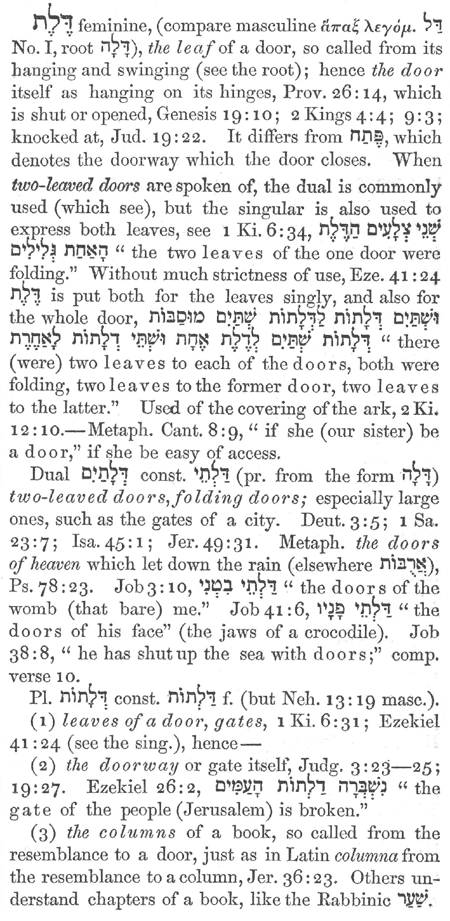
\includegraphics[width=8cm]{deleth_h1817}


The root of that has the concept of "deliver"
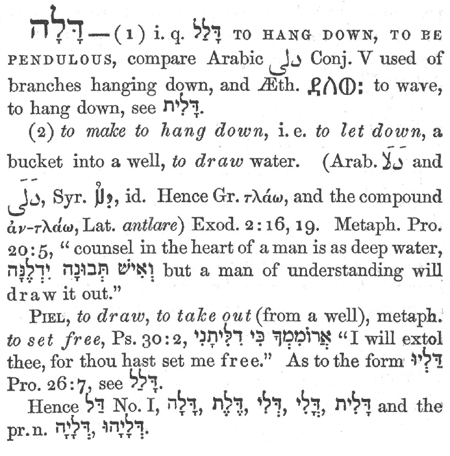
\includegraphics[width=8cm]{dala_h1802}

 daw-law'; a primitive root (compare H1809); properly, to dangle, i.e. to let down a bucket (for drawing out water); figuratively, to deliver:
 \begin{hebrew}
 דָּלָה        
 \end{hebrew}
—draw (out), enough, lift up.

blueletterbible.org Bible has this for G2374 which is the Greek word used for "door" in Deuteronomy 15:17
\begin{quote}
in a parable or metaphor

the door through which sheep go in and out, the name of him who brings salvation to those who follow his guidance

"an open door" is used of the opportunity of doing something

the door of the kingdom of heaven (likened to a palace) denotes the conditions which must be complied with in order to be received into the kingdom of God:
\url{https://www.blueletterbible.org/lang/Lexicon/Lexicon.cfm?strongs=G2374&t=KJV}
\end{quote}


I should also note that the places in the Torah where blood is on the earlobes is where there is a change from a lower to higher status. The priest becomes able to serve in the temple and the leprous person is allowed to come back in the camp:

\begin{quote}
“I am the door” in John 10: “Truly, truly, I say to you, I am the door of the sheep”, and again, “I am the door. If anyone enters by me, he will be saved and will go in and out and find pasture”.

We find that earlobes also feature in two other significant places in the Torah – in the consecration of priests, and the cleansing of lepers: Leviticus 8:1

“Now this is what you shall do to them to consecrate them, that they may serve me as priests… you shall kill the ram and take part of its blood and put it on the tip of the right ear of Aaron and on the tips of the right ears of his sons, and on the thumbs of their right hands and on the great toes of their right feet, and throw the rest of the blood against the sides of the altar.”

Levticus 14:1-4 “The Lord spoke to Moses, saying, “This shall be the law of the leprous person for the day of his cleansing… the priest shall command them to take for him who is to be cleansed two live clean birds and cedarwood and scarlet yarn and hyssop…”

Scarlet yarn? Like the colour of blood? And hyssop, you say? Like they used to paint the blood on the doorframes on Passover night? Interesting…

It continues, v14-20: “The priest shall take some of the blood of the guilt offering, and the priest shall put it on the lobe of the right ear of him who is to be cleansed and on the thumb of his right hand and on the big toe of his right foot. Then the priest shall take some of the log of oil and pour it into the palm of his own left hand and dip his right finger in the oil that is in his left hand and sprinkle some oil with his finger seven times before the Lord. And some of the oil that remains in his hand the priest shall put on the lobe of the right ear of him who is to be cleansed and on the thumb of his right hand and on the big toe of his right foot, on top of the blood of the guilt offering. And the rest of the oil that is in the priest’s hand he shall put on the head of him who is to be cleansed… Thus the priest shall make atonement for him, and he shall be clean.”

\url{oneforisrael.org}
\end{quote}


Karel Van Der Toorn makes an additional connection related to the ceremony of the servant at the doorpost:
\begin{quote}
The connection between the ancestors and the family inheritance is well `attested in the Hebrew Bible. The family inheritance (nahala) is the 'inheritance of the fathers (nahalat abor 1 Kgs 21:3) It is not to be sold or exchanged (1 Kgs 21:1-4). A paralel to the expression 'inheritance of the fathers' (nahalat abot) is the construction 'inheritance of the gods' (nahalat elehim, 2 Sam 14:16). In Emar, the term 'gods' can refer to the ancestors. The same phenomenon occurs in Ugaritic texts (KTU1.6 vi 45-49). Also in the Hebrew Bible, there are at least two instances where elohim must be understood as a reference to the spirits of the dead (1 Sam 28:13; Isa 8:19) Theodore Lewis suggests it must be so understood as well in the expression nahalat 'elohim; the expression stands for 'the ancestral estate.'21

The possibility that the term 'gods' might in fact refer to the spirits of the dead opens up new avenues of investigation. One of the earliest--if not the earliest--parts of the Hebrew legal corpus is the so-called Covenant Code (Exod 20:22-23:33, the oldest section of which is 21:1-22:16). It contains the rule that the slave who waives his right of manumission and enters his master's household for good is to be brought 'to the gods;' here his ear is to be pierced by his master (Exod 21:6). A glossator has added that the man shall be brought 'to the door or to the doorpost,' perhaps the place where the 'gods' were thought to reside. These 'gods,' I submit, are in fact the family ancestors.22 What we have here is a rite of passage in a case of adoption. The new member of the family is presented to its forebears; he is bodily marked, and henceforth indissolubly part of the family.23 Whether the ancestors were physically represented by images cannot be decided on the basis of this text alone. The possibility cannot be ruled out, since it is likely that the teraphim, known from other sources, were in fact ancestor statuettes.24
\end{quote}

He goes on to mention the profession of innocence in Deut 26:14 suggesting that ancestor worship was known to Israelites and practiced at least occasionally well up to Hellenistic Palestine: (Tob 4:17; Sir 30:18) David makes an excuse for not being at Saul's table via a regular sacrificial meal (zebah) of the clan (mispaha) that was partly funerary which is corroborated "oblique[ly]" in the events of 1 Sam 10:1-16. Where there are two men by Rachel's tomb and three men go up to "elohim" at bethel. Karel suggest that the events are situated in the new moon or "interlunium" (cf. theMesopotamian bubbulu) where according to tradition families would gather for sacrificial purposes "1 Sam 20:5,18-19,24,27,34" and that since the tombs are mentioned that it may have some connection with this ritual. Here I would disagree. I think God replaced the cult of the ancestors but I think his observations that these practices may have been used to worship God shows some evidence for that.

Gen 31 and 1 Samuel 19 gives evidence for the teraphim being defined as "household gods." This conclusion agrees with the usual rendering "terapim" by the Targums and the Vulgate (nomally idola, see Judg 17:5, "et fecit ephod ac therafin id est vestem sacr-dotalem et idola" as well as Young's literal translation of these verses. In Judges 18:24 Micah claims that the Danites have taken "my god which I have made." If we understand as the elohay as the common plural "my gods", the designation would include the ephod and the teraphim. In Gen 31:30 Laban calls the stolen teraphim his "gods." (see again the previously mentioned 1 Sam 28:13) To Karel again:
\begin{quote}
In the ancient Near East, ancestors were believed to be endowed with powers denied to the living. They were, so to speak, semigods. Thus, Akkadian texts do sometimes speak ilu, "god," in connection with a ghost,26 and an Ugaritic hymn to Shapash, set within the Baal Cycle, puts the ilm in parallelism with mtm.27 As semidivine beings, the Israelite dead could at times be subsumed under the category of "elohim," without losing their human character. Therefore, while the teraphim are certaily numinous images, they need not have represented gods strictly speaking. For the time being we can only say that the teraphim were "cultic figurines" or "religious statuettes."
%insert reference to Karel Van Der Toorn
\end{quote}

For instance:
\begin{quote}
As to the man Micah, he hath a house of gods, and he maketh an ephod, and teraphim, and consecrateth the hand of one of his sons, and he is to him for a priest; (Judges 17:5)
\end{quote}

According to Isaiah 8:19 the Israelites used to speak of the "dead" (metim) as "gods."
\begin{quote}
And when they say unto you, 'Seek unto those having familiar spirits, And unto wizards, who chatter and mutter, Doth not a people seek unto its God? -- For the living unto the dead! (Isaiah 8:19)
\end{quote}



\begin{hebrew}
מחקר המקבילות במסגרת מחקר המקרא: לשם מה?    
\end{hebrew}
 \ PARALLELS IN BIBLICAL RESEARCH: PURPOSES OF COMPARISON\
KAREL VAN DER TOORN and קרל ון דר טורן

\url{https://www.jstor.org/stable/23535740?seq=1#page_scan_tab_contents}


%Family Religion in Babylonia, Ugarit and Israel: Continuity and Changes in ...
%By K. Van Der Toorn

%The Body as Property: Physical Disfigurement in Biblical Law
%By Sandra Jacob (this contains a passage that I was unable to screenshot before the passage on the ex 26:1 and deut 15)


%https://books.google.com/books?id=efMPAwAAQBAJ&pg=PA193&lpg=PA193&dq=pierce+his+ear+with+an+awl+and+adoption&source=bl&ots=KQ7tjCB47F&sig=ACfU3U3Ugoa5rdAzzWk9pRJ8Bp8ZwH1xIA&hl=en&sa=X&ved=2ahUKEwjapKC9tMniAhVEHqwKHa7GAGIQ6AEwEHoECC4QAQ#v=onepage&q=pierce%20his%20ear%20with%20an%20awl%20and%20adoption&f=false


Finally we can also observe that the door and post were where they stationed gods:

8 And behind the door, and the post, Thou hast set up thy memorial, For from Me thou hast removed, and goest up, Thou hast enlarged thy couch, And dost covenant for thyself among them, Thou hast loved their couch, the station thou sawest (Isaiah 57:8)


\
\begin{quote}
An example of legal practice that is corroborated by a variety of sources, Israelite homicide law may be examined as a complex nexus of private negotiation, procedural guidelines, cultic requirements, and official state intervention. According to Pamela Barmash, rather than a “paroxysm of rage,” blood feud ought best be understood as “a legal mechanism that both assures the redress of wrongs and controls the violence to a level tolerable in a community … [I]t is local in nature, and … rule-bound.”29 She goes on to describe blood-feud in ancient Israel as follows:
\begin{quote}

The victim’s family undertook the initiative in punishing a homicide, but there were qualifications. Only the slayer was subject to action, not anyone else, whether having a connection to him or not. Apparently only a specific member of the victim’s family, go’el hadam [the “blood avenger”], had the right to kill the slayer with impunity. The cities of refuge acted as a check on the right of [the blood avenger] to kill the slayer with impunity. He could not kill a slayer while the slayer was within the city of refuge (Num. 35:12; Deut. 19:5; Josh. 20:5). Second, once the slayer had entered the city of refuge, he was subject to trial to determine whether it was an intentional or accidental homicide (Num. 35:24; Deut. 19:12). This decision limited the ability of [the blood avenger] to effect vengeance because if the slayer was judged to be an accidental killer, he was permitted to stay in the city of refuge safe from the avenger. Only if the slayer was determined to be an intentional killer was he handed over to the avenger for execution. Indeed, biblical texts manifest anxiety over the possibility that [the blood avenger] might kill an accidental killer because he could kill any slayer with impunity outside the city of refuge (Deut. 19:6).30 
\end{quote}

Within this legal mechanism to remedy homicide, then, are a variety of styles of jurisprudence. We see the “customary law” of Israelite clan life, which relied on immediate but limited vengeance for the victim’s family. Identification of the killer is not presented as an issue; we might presume that in small communities, the identity of the killer was most often known to all and not the vexed issue it is in murder mysteries today.31 We may also note the presence of “cities of refuge,” which may have been connected to a local shrine or altar32 and provide a kind of divine protection for the slayer who is believed to have killed without intent. These “cities of refuge” (or the altar itself, as described in Exod 21:13–14) reveal how religious or cultic institutions might function legally in some respects. The trial, then, is apparently only required for a slayer who has fled to a city of refuge, and therefore more “official” oversight in respect of the sanctions for homicide – identifying the killer’s intent and motivations, the murder weapon used (bare hands or iron tool, for example33), the history (or lack thereof) of enmity between the killer and the victim – is reserved for only certain cases, but it is available nonetheless. Barmash clarifies that the trial is conducted normally by local officials or elders; the monarchy and/or the central sanctuary do not intervene other than in truly exceptional circumstances.34 Thus, the procedure for blood feud appears to be both informal and rule bound; privately negotiated and navigated, but with the possibility that central authorities can be petitioned or invoked if a case warrants it.
\url{https://www.cambridge.org/core/books/cambridge-companion-to-judaism-and-law/law-in-biblical-israel/1CD3E55866319000E150DCD3934C9191/core-reader}
\end{quote}

So I think Exodus 21:20-21 could be explained by the fact that the legal system may have been more distributed in that day, so in this case the person who had the servant is acting as the government. Some evidence for this is that you wouldn't often post legal statutes on the doors of your house unless you were responsible for enforcing them (this is something you normally would find in court rooms)


\begin{quote}
7 and thou hast repeated them to thy sons, and spoken of them in thy sitting in thine house, and in thy walking in the way, and in thy lying down, and in thy rising up,
8 and hast bound them for a sign upon thy hand, and they have been for frontlets between thine eyes,
9 and thou hast written them on door-posts of thy house, and on thy gates. (Deuteronomy 6:7-9)
\end{quote} 

This isn't conclusive because maybe God just wanted everyone to know the legal system very well so that they wouldn't infringe upon it. We also have the right of househoulds to own land and for that land to always return to them during the jubilee year. There seems to a be connection between this and the laws governing servants as well:
\begin{quote}
23 `And the land is not sold -- to extinction, for the land [is] Mine, for sojourners and settlers [are] ye with Me;

24 and in all the land of your possession a redemption ye do give to the land.

25 `When thy brother becometh poor, and hath sold his possession, then hath his redeemer who is near unto him come, and he hath redeemed the sold thing of his brother;

26 and when a man hath no redeemer, and his own hand hath attained, and he hath found as sufficient [for] its redemption,

27 then he hath reckoned the years of its sale, and hath given back that which is over to the man to whom he sold [it], and he hath returned to his possession.

28 `And if his hand hath not found sufficiency to give back to him, then hath his sold thing been in the hand of him who buyeth it till the year of jubilee; and it hath gone out in the jubilee, and he hath returned to his possession.

29 `And when a man selleth a dwelling-house [in] a walled city, then hath his right of redemption been until the completion of a year from its selling; days -- is his right of redemption;

30 and if it is not redeemed until the fulness to him of a perfect year, then hath the house which [is] in a walled city been established to extinction to the buyer of it, to his generations; it goeth not out in the jubilee;

31 and a house of the villages which have no wall round about, on the field of the country is reckoned; redemption is to it, and in the jubilee it goeth out.

32 `As to cities of the Levites -- houses of the cities of their possession -- redemption age-during is to the Levites;

33 as to him who redeemeth from the Levites, both the sale of a house and the city of his possession have gone out in the jubilee, for the houses of the cities of the Levites are their possession in the midst of the sons of Israel.

34 And a field, a suburb of their cities, is not sold; for a possession age-during it [is] to them.

35 `And when thy brother is become poor, and his hand hath failed with thee, then thou hast kept hold on him, sojourner and settler, and he hath lived with thee;

36 thou takest no usury from him, or increase; and thou hast been afraid of thy God; and thy brother hath lived with thee;

37 thy money thou givest not to him in usury, and for increase thou givest not thy food;

38 I [am] Jehovah your God, who hath brought you out of the land of Egypt, to give to you the land of Canaan, to become your God.

39 `And when thy brother becometh poor with thee, and he hath been sold to thee, thou dost not lay on him servile service;

40 as an hireling, as a settler, he is with thee, till the year of the jubilee he doth serve with thee, --

41 then he hath gone out from thee, he and his sons with him, and hath turned back unto his family; even unto the possession of his fathers he doth turn back.

42 `For they [are] My servants, whom I have brought out from the land of Egypt: they are not sold [with] the sale of a servant;

43 thou rulest not over him with rigour, and thou hast been afraid of thy God.

44 `And thy man-servant and thy handmaid whom thou hast [are] of the nations who [are] round about you; of them ye buy man-servant and handmaid,

45 and also of the sons of the settlers who are sojourning with you, of them ye buy, and of their families who [are] with you, which they have begotten in your land, and they have been to you for a possession;

46 and ye have taken them for inheritance to your sons after you, to occupy [for] a possession; to the age ye lay service upon them, but upon your brethren, the sons of Israel, one with another, thou dost not rule over him with rigour.

47 `And when the hand of a sojourner or settler with thee attaineth [riches], and thy brother with him hath become poor, and he hath been sold to a sojourner, a settler with thee, or to the root of the family of a sojourner,

48 after he hath been sold, there is a right of redemption to him; one of his brethren doth redeem him,

49 or his uncle, or a son of his uncle, doth redeem him, or any of the relations of his flesh, of his family, doth redeem him, or -- his own hand hath attained -- then he hath been redeemed.

50 `And he hath reckoned with his buyer from the year of his being sold to him till the year of jubilee, and the money of his sale hath been by the number of years; as the days of an hireling it is with him.

51 `If yet many years, according to them he giveth back his redemption [money], from the money of his purchase.

52 `And if few are left of the years till the year of jubilee, then he hath reckoned with him, according to his years he doth give back his redemption [money];

53 as an hireling, year by year, he is with him, and he doth not rule him with rigour before thine eyes.

54 `And if he is not redeemed in these [years], then he hath gone out in the year of jubilee, he and his sons with him.

55 For to Me [are] the sons of Israel servants; My servants they [are], whom I have brought out of the land of Egypt; I, Jehovah, [am] your God. (Leviticus 25:23-55)
\end{quote} 

God not only says that the sons of Israel belongs to him as servants but that the land ultimately belongs to him and that's why it also cannot be sold permenantly: Leviticus 25:23. This goes along with the idea of the household and clan based legal structure that is talked about here by Keith Reeves:

\begin{quote}
Within the nation we find the tribes, which according to Numbers 26:52-56 received initial land allotments according to size. The tribes, in turn, are composed of clans – larger family units that might comprise a village or a region. The clans had a vital social function, which we will discuss below.

Within the clans was the most basic unit, the “father’s house.” This is headed by the “father,” the oldest living patriarch of the family. Children, grandchildren, and great-grandchildren are all under the authority of the father. The father’s house could be a fairly large unit, comprised of more than 50 people.

The father’s house is where the ownership of land actually occurred. Today, individuals own land, either singly or jointly. In Israel, land belonged to a father’s house rather than to any individual or set of individuals.

The father’s house was therefore a vital link both to the land and to Yahweh for the individuals in the house. Ultimately, the land belonged to Yahweh (Leviticus 25:23). But it was “owned” in a more secondary sense, and managed, by the father’s house.

Thus, the laws in Israel were designed to maintain the integrity of the father’s house and its connection with the land. There are many such laws, but we can only touch on a few. \url{https://oikonomianetwork.org/2015/11/family-land-and-household-in-the-old-testament/}
\end{quote}

He then goes on to mention the implied clan based responsibility for vengence in 2 Samuel 14:6 as well as their responsibility for redeeming indentured sevants and the land: Leviticus 25:47-52, Leviticus 25:23-28. For household based rule he mentions the law of the rebellious son in Deuteronomy 21:18-21 as well as the Levirate marriage in Deuteronomy 25:5-10, the law of the man who does not build up his brother's house Deuteronomy 25:9, the story of Onan Genesis 38:8-10 and the story of Ruth's default redeemer: Ruth 4:1-6 which when he refuses passes to Boaz. He argues that the reason the default redeemer refuses is not only would he have to pay for the field but that the field that Noami's husband (Elimelech) sold before he moved to Moab (he would have to redeem it) but that it would pass to Ruth's firstborn son. The firstborn would be Elimelech's legal heir and that this gives us insight into why the villagers say: “and let thy house be as the house of Pharez (whom Tamar bare to Judah), of the seed which Jehovah doth give to thee of this young woman.'” (Ruth 4:12). Perez was a twin (Genesis 38:39) who also had twins. The firstborn child of Ruth would legally be Elimelech’s heir, whereas the second born would be Boaz’s heir. 

In the second article \url{https://oikonomianetwork.org/2015/12/households-and-economic-injustice-in-the-old-testament/} professor Reeves argues that the monarchy (which we can see was not God's intention from 1 Samuel 8:1-18) was a direct challenge to the clan and household based authority structure:

\begin{quote}
And it cometh to pass, when Samuel [is] aged, that he maketh his sons judges over Israel.

2 And the name of his first-born son is Joel, and the name of his second Abiah, judges in Beer-Sheba:

3 and his sons have not walked in his ways, and turn aside after the dishonest gain, and take a bribe, and turn aside judgment.

4 And all the elders of Israel gather themselves together, and come in unto Samuel to Ramath,

5 and say unto him, `Lo, thou hast become aged, and thy sons have not walked in thy ways; now, appoint to us a king, to judge us, like all the nations.'

6 And the thing is evil in the eyes of Samuel, when they have said, `Give to us a king to judge us;' and Samuel prayeth unto Jehovah.

7 And Jehovah saith unto Samuel, `Hearken to the voice of the people, to all that they say unto thee, for thee they have not rejected, but Me they have rejected, from reigning over them.

8 According to all the works that they have done from the day of My bringing them up out of Egypt, even unto this day, when they forsake Me, and serve other gods -- so they are doing also to thee.

9 And now, hearken to their voice; only, surely thou dost certainly protest to them, and hast declared to them the custom of the king who doth reign over them.'

10 And Samuel speaketh all the words of Jehovah unto the people who are asking from him a king,

11 and saith, `This is the custom of the king who doth reign over you: Your sons he doth take, and hath appointed for himself among his chariots, and among his horsemen, and they have run before his chariots;

12 also to appoint for himself heads of thousands, and heads of fifties; also to plow his plowing, and to reap his reaping; and to make instruments of his war, and instruments of his charioteer.

13 `And your daughters he doth take for perfumers, and for cooks, and for bakers;

14 and your fields, and your vineyards, and your olive-yards -- the best -- he doth take, and hath given to his servants.

15 And your seed and your vineyards he doth tithe, and hath given to his eunuchs, and to his servants.

16 And your men-servants, and your maid-servants, and your young men -- the best, and your asses, he doth take, and hath prepared for his own work;

17 your flock he doth tithe, and ye are to him for servants.

18 And ye have cried out in that day because of the king whom ye have chosen for yourselves, and Jehovah doth not answer you in that day.' (1 Samuel 8:1-18)
\end{quote} 

He continues by observing that in 1 Kings 4:7 that Solomon had 12 officials over Israel and each official was to provide food for the king and his household for one month of the year and that solomon conscripted many people into forced labor. (this would seem to infringe on the power of the households and clans) Also king Ahab and Jezebeel steal a vineyard from Naboth in 1 Kings 21:1-16 which goes against the family ownership structure we see outlined in the law. It is interesting that Ahab goes hom sad when Naboth refuses to sell his vineyard and it is Jezebeel who orchestrates the theft causing people to fasely accuse him of cursing God and the king. This implies that the household land ownship princples were not even supposed to usurped by the monarchy and this may be partially what draws the ire of the prophets in 1 Kings 21:17–19 for "killing and taking possession." Professor Reeves goes on to write:
\begin{quote}
This is a common indictment by Amos, Isaiah, and Micah. Additional critiques of land seizure can be found in Isaiah 3:13–15; 5:8–10; 10:1–2; Hosea 5:10; and Micah 2:1–4, 8–9.

The passage from Micah is especially illustrative. It demonstrates that the land and the presence of Yahweh are intimately connected. If you drive the women out of the land, you remove their children from Yahweh’s glory. \url{https://oikonomianetwork.org/2015/12/households-and-economic-injustice-in-the-old-testament/}
\end{quote} 

Another part I found interesting in his first article was the application this has for today:
\begin{quote}
This is much more than just interesting history. The family unit is as important to economics and social order today as it was in ancient Israel. We no longer have a land-based economy, so land as such is not the key factor now. But the family is still vitally connected to the economy. Nick Schulz, in Home Economics: the Consequences of Changing Family Structure, details the destructive consequences of the breakdown of the family in America. Wayne Grudem and Barry Asmus, in their book The Poverty of Nations, include “Laws that give protection and positive economic incentives to stable family structures” as one of the factors that help nations overcome poverty (p. 256-257).\url{https://oikonomianetwork.org/2015/11/family-land-and-household-in-the-old-testament/}
\end{quote} 


However, to bring us back to the discussion, I should note that it wasn't a household system based completely on patriachy as Carol Meyers observes:
\begin{quote}
. . . 
 Abigail (1Sam 25), a woman with access to resources, uses them cleverly to save her household; she acts without consulting her husband and gives orders to the household staff. The Shunammite woman (2Kgs 4:8-37; 2Kgs 8:1-6) also acts autonomously in inviting a prophet to her house, reconfiguring household space, moving her family to escape a drought, and negotiating with the king about family property. Micah’s mother (Judg 17) and the “strong woman” (NRSV “capable wife”) of Proverbs (Prov 31:10-31) show similar agency. In addition, information in the Hebrew Bible calls into question the idea that women were excluded from community life. About twenty different community roles were held by women. These included leadership positions, for example: Deborah, prophet and judge (Judg 4-5); Miriam, prophet (Exod 15:20-21); and the woman of Abel of Beth-maacah, sage (2Sam 20:14-22). This challenge to patriarchy as an appropriate term for the Israelites does not mean that women and men were equal. Men still dominated, for example, in most community roles. . . .\url{https://www.bibleodyssey.org/en/passages/related-articles/patriarchy-and-the-hebrew-bible}
\end{quote}


The Cambridge Companion to Judaism and Law concures with Reeves's findings on the decentralized nature of biblical law while also mentioning the role of the heads of households:

\begin{quote}
Legal Practice in Ancient Israel
The question of whether decentralized, premodern societies had “law” or simply “norms” or “customs” has not yet been fully settled among legal theorists, legal sociologists, or legal anthropologists. For our purposes, we may define law rather broadly, following the lead of legal theorist Lon Fuller: “law is the enterprise of subjecting human conduct to the governance of rules.”2 Seen through this wide lens, it is probable, then, that ancient Israelite societies had some measure of a “legal enterprise”: that elders, heads of households, priests, officials, and monarchs were tasked to ensure harmony among families and communities by resolving disputes and intervening when traditional rules were violated. Though they were not expected to adhere strictly to a code of law, there was, most likely, a body of tradition that provided the bases for social justice – and just decision making – that persisted throughout the generations within ancient Israel.3 \url{https://www.cambridge.org/core/books/cambridge-companion-to-judaism-and-law/law-in-biblical-israel/1CD3E55866319000E150DCD3934C9191/core-reader}
\end{quote} 

To bring us back to the controvery surrounding Exodus 21:20-21 and the corporal punishment of a servant we should observe that Legal systems with corporal punishment are implemented today by the well educated and technologically advanced country of Singapore: "The Government of Singapore has defended the punishment as a traditional part of the country's legal system." \url{https://www.nytimes.com/1994/06/26/us/us-student-tells-of-pain-of-his-caning-in-singapore.html} Obviously this is not an argument of it's morality but it should give us some pause if we think of corporal punishment as being primitive. In addition, if the reading of the majority of translations is to be accepted \url{http://biblehub.com/exodus/21-21.htm} this must be a case where the cause of death was uncertain as verse 26 implies that any significant damage would have them avenged as a free person. If he dies as a free man then he is avenged as a free man so if you beat your servant and cause significant damage and he continues for a few days before he dies this would still result in you being tried for murder. This law seems to only prevent trial for murder when there is no evidence that the beating caused the death of the servant.


\section{Concubines}

A common argument I find is that concubines were throw away women without any legal standing as wives and were bassically consistent sexual partners. I ask the reader to look at the complete usage of the word concubine in the Bible, luckily with only one strong's number:

Complete list of the occurrences of the word "concubine." The following verses are in the KJV:

\begin{lstlisting}
Gen 22:24
And his concubine, H6370 whose name was Reumah, she bare also Tebah, and Gaham, and Thahash, and Maachah.


Gen 25:6
But unto the sons of the concubines, H6370 which Abraham had, Abraham gave gifts, and sent them away from Isaac his son, while he yet lived, eastward, unto the east country.


Gen 35:22
And it came to pass, when Israel dwelt in that land, that Reuben went and lay with Bilhah his father's concubine: H6370 and Israel heard it. Now the sons of Jacob were twelve:


Gen 36:12
And Timna was concubine H6370 to Eliphaz Esau's son; and she bare to Eliphaz Amalek: these were the sons of Adah Esau's wife.


Jdg 8:31
And his concubine H6370 that was in Shechem, she also bare him a son, whose name he called Abimelech.


Jdg 19:1
And it came to pass in those days, when there was no king in Israel, that there was a certain Levite sojourning on the side of mount Ephraim, who took to him a concubine H6370 out of Bethlehemjudah.


Jdg 19:2
And his concubine H6370 played the whore against him, and went away from him unto her father's house to Bethlehemjudah, and was there four whole months.


Jdg 19:9
And when the man rose up to depart, he, and his concubine, H6370 and his servant, his father in law, the damsel's father, said unto him, Behold, now the day draweth toward evening, I pray you tarry all night: behold, the day groweth to an end, lodge here, that thine heart may be merry; and to morrow get you early on your way, that thou mayest go home.


Jdg 19:10
But the man would not tarry that night, but he rose up and departed, and came over against Jebus, which is Jerusalem; and there were with him two asses saddled, his concubine H6370 also was with him.


Jdg 19:24
Behold, here is my daughter a maiden, and his concubine; H6370 them I will bring out now, and humble ye them, and do with them what seemeth good unto you: but unto this man do not so vile a thing.


Jdg 19:25
But the men would not hearken to him: so the man took his concubine, H6370 and brought her forth unto them; and they knew her, and abused her all the night until the morning: and when the day began to spring, they let her go.


Jdg 19:27
And her lord rose up in the morning, and opened the doors of the house, and went out to go his way: and, behold, the woman his concubine H6370 was fallen down at the door of the house, and her hands were upon the threshold.


Jdg 19:29
And when he was come into his house, he took a knife, and laid hold on his concubine, H6370 and divided her, together with her bones, into twelve pieces, and sent her into all the coasts of Israel.


Jdg 20:4
And the Levite, the husband of the woman that was slain, answered and said, I came into Gibeah that belongeth to Benjamin, I and my concubine, H6370 to lodge.


Jdg 20:5
And the men of Gibeah rose against me, and beset the house round about upon me by night, and thought to have slain me: and my concubine H6370 have they forced, that she is dead.


Jdg 20:6
And I took my concubine, H6370 and cut her in pieces, and sent her throughout all the country of the inheritance of Israel: for they have committed lewdness and folly in Israel.


2Sa 3:7
And Saul had a concubine, H6370 whose name was Rizpah, the daughter of Aiah: and Ishbosheth said to Abner, Wherefore hast thou gone in unto my father's concubine? H6370


2Sa 5:13
And David took him more concubines H6370 and wives out of Jerusalem, after he was come from Hebron: and there were yet sons and daughters born to David.


2Sa 15:16
And the king went forth, and all his household after him. And the king left ten women, which were concubines, H6370 to keep the house.


2Sa 16:21
And Ahithophel said unto Absalom, Go in unto thy father's concubines, H6370 which he hath left to keep the house; and all Israel shall hear that thou art abhorred of thy father: then shall the hands of all that are with thee be strong.


2Sa 16:22
So they spread Absalom a tent upon the top of the house; and Absalom went in unto his father's concubines H6370 in the sight of all Israel.


2Sa 19:5
And Joab came into the house to the king, and said, Thou hast shamed this day the faces of all thy servants, which this day have saved thy life, and the lives of thy sons and of thy daughters, and the lives of thy wives, and the lives of thy concubines; H6370


2Sa 20:3
And David came to his house at Jerusalem; and the king took the ten women his concubines, H6370 whom he had left to keep the house, and put them in ward, and fed them, but went not in unto them. So they were shut up unto the day of their death, living in widowhood.


2Sa 21:11
And it was told David what Rizpah the daughter of Aiah, the concubine H6370 of Saul, had done.


1Ki 11:3
And he had seven hundred wives, princesses, and three hundred concubines: H6370 and his wives turned away his heart.


1Ch 1:32
Now the sons of Keturah, Abraham's concubine: H6370 she bare Zimran, and Jokshan, and Medan, and Midian, and Ishbak, and Shuah. And the sons of Jokshan; Sheba, and Dedan.


1Ch 2:46
And Ephah, Caleb's concubine, H6370 bare Haran, and Moza, and Gazez: and Haran begat Gazez.


1Ch 2:48
Maachah, Caleb's concubine, H6370 bare Sheber, and Tirhanah.


1Ch 3:9
These were all the sons of David, beside the sons of the concubines, H6370 and Tamar their sister.


1Ch 7:14
The sons of Manasseh; Ashriel, whom she bare: (but his concubine H6370 the Aramitess bare Machir the father of Gilead:


2Ch 11:21
And Rehoboam loved Maachah the daughter of Absalom above all his wives and his concubines: H6370 (for he took eighteen wives, and threescore concubines; H6370 and begat twenty and eight sons, and threescore daughters.)


Est 2:14
In the evening she went, and on the morrow she returned into the second house of the women, to the custody of Shaashgaz, the king's chamberlain, which kept the concubines: H6370 she came in unto the king no more, except the king delighted in her, and that she were called by name.


Sng 6:8
There are threescore queens, and fourscore concubines, H6370 and virgins without number.


Sng 6:9
My dove, my undefiled is but one; she is the only one of her mother, she is the choice one of her that bare her. The daughters saw her, and blessed her; yea, the queens and the concubines, H6370 and they praised her.


Eze 23:20
For she doted upon their paramours, H6370 whose flesh is as the flesh of asses, and whose issue is like the issue of horses.
\end{lstlisting}

\section{Keturah}
First off lets put an end to the myth that concubines weren't also wives:
Gen 25:1
Then again Abraham took a wife, and her name was Keturah. H6989

Gen 25:4
And the sons of Midian; Ephah, and Epher, and Hanoch, and Abida, and Eldaah. All these were the children of Keturah. H6989

1Ch 1:32
Now the sons of Keturah, H6989 Abraham's concubine: she bare Zimran, and Jokshan, and Medan, and Midian, and Ishbak, and Shuah. And the sons of Jokshan; Sheba, and Dedan.

Also it was considered horrific to David when Absalom slept with David's concubines:

\begin{quote}
21 And Ahithophel saith unto Absalom, `Go in unto the concubines of thy father, whom he left to keep the house, and all Israel hath heard that thou hast been abhorred by thy father, and the hands of all who [are] with thee have been strong.'

22 And they spread out for Absalom the tent on the roof, and Absalom goeth in unto the concubines of his father before the eyes of all Israel.

23 And the counsel of Ahithophel which he counselled in those days [is] as [when] one inquireth at the word of God; so [is] all the counsel of Ahithophel both to David and to Absalom.
(2 Samuel 2:21-23)
\end{quote}

Also the sons and daughters of concubines and wives were not differentiated by the text:

And Rehoboam loveth Maachah daughter of Absalom above all his wives and his concubines -- for eighteen wives he hath taken, and sixty concubines -- and he begetteth twenty and eight sons, and sixty daughters. (2 Ch 11:21)
\begin{quote}
30 and to Gideon there have been seventy sons, coming out of his loin, for he had many wives;
31 and his concubine, who [is] in Shechem, hath born to him -- even she -- a son, and he appointeth his name Abimelech. (Judges 8:30-31)
\end{quote}

Although there is some evidence that Abraham may have differentiated their sons from his:
\begin{quote}
5 And Abraham giveth all that he hath to Isaac;
6 and to the sons of the concubines whom Abraham hath, Abraham hath given gifts, and sendeth them away from Isaac his son (in his being yet alive) eastward, unto the east country. (Gen 25:5-6)
\end{quote}

The death and molestation of a single concubine could cause all of Israel to turn against one of it's own tribes in a massive bloody conflict even after the concubine had commited whoredom against her husband. This shows concubines were valued and were not just considered throw away women:

\begin{quote}
29 and cometh in unto his house, and taketh the knife, and layeth hold on his concubine, and cutteth her in pieces to her bones -- into twelve pieces, and sendeth her into all the border of Israel.
30 And it hath come to pass, every one who seeth hath said, `There hath not been -- yea, there hath not been seen like this, from the day of the coming up of the sons of Israel out of the land of Egypt till this day; set your [heart] upon it, take counsel, and speak.'
1 And all the sons of Israel go out, and the company is assembled as one man, from Dan even unto Beer-Sheba, and the land of Gilead, unto Jehovah, at Mizpeh.

2 And the chiefs of all the people, of all the tribes of Israel, station themselves in the assembly of the people of God, four hundred thousand footmen drawing sword.

3 And the sons of Benjamin hear that the sons of Israel have gone up to Mizpeh. And the sons of Israel say, `Speak ye, how hath this evil been?'

4 And the man, the Levite, husband of the woman who hath been murdered, answereth and saith, `Into Gibeah (which [is] to Benjamin) I have come, I and my concubine, to lodge;

 (Jdg 19:29-20:4)
\end{quote}

Notice it indeed calls him her "husband" literally "the man, the levite, the man of the woman [who was] murdered"
\begin{hebrew}
הָאִישׁ הַלֵּוִי אִישׁ הָאִשָּׁה הַנִּרְצָחָ֖ה

\end{hebrew}
Since there is no direct word for husband or for sex in hebrew those concepts are gathered by context and possession. The septuagint says [3answered 1the 2man], the Levite, the husband of the woman having been murdered
literally: "[3answered 1the 2man], the Levite, the man of the woman having been murdered"

\begin{greek}
 ἀπεκρίθη ὁ ἀνὴρ ὁ Λευίτης ὁ ἀνὴρ τῆς γυναικὸς τῆς πεφονευμένης
\end{greek}


Concubines were considered to be sexually sinning if they slept with another man just like wives:

And his concubine H6370 played the whore against him, and went away from him unto her father's house to Bethlehemjudah, and was there four whole months. (Jdg 19:2)


\section{Comparison of ancient laws}


Some argue that the only reason the Bible prohibited premarital sex is because of the need to legitimise the descent of the children. This is partially based on the idea of a patriachal culture which we have seen is an inapt description of ancient Israel. There is evidence that people believed biological descent to be important in the Old Babylonian period\cite{son of p} which would be very roughly (hundreds of years) within the time that the law was given and the later Neo-Babylonian period. \cite{exorcist in emar} However, there are several examples that show this idea's poverty in explaining the death penalty for adultery. First, if the sin was only against the husband (presumably the person to whom the descent mattered) why couldn't the husband pardon the woman? Also why was it death? Surely not knowing the descent of someone shouldn't be cause for death even in a patriarchal culture. The woman at least should be able to redeem herself if she bears the husband more children (I'm speaking like I imagine a patriarchal person would speak) It would be no use to the husband if he now had a child of uncertain descent and now he had to kill off the provider of his children. Wouldn't it make more sense (even from the selfish perspective of the husband) to preserve his wife so he could have more children in the future unless he decided she was totally untrustworthy. Why isn't there a provision for adultury for women who are sterile? or for women who's husbands were sterile? (she couldn't be accused of trying to pass off a child as their husband's) 





\medskip
\begin{thebibliography}{56}
\bibitem{son of p} 
An Old Babylonian agreement concerned a woman who already had a son by a man named P., and with this son `she entered the house of M.'. So she was a widow who had begun to cohabit. When subsequently she was `seized by the seizure of a god', meaning that she had become seriously ill, she applied to the judges, who `pronounced her departure'. That means that she had permission (or
was obliged) to divorce. From the rest of the text it would appear that her own son had no right of inheritance in his new surroundings. 

\begin{quote}
The son himself said, I am the son of P. and you are not my father.
\end{quote}
\url{http://www.oapen.org/download?type=document&docid=650050}


\bibitem{exorcist in emar}
In Chapter 5 we saw that an exorcist in Emar married a widow with a son as his
second wife, and that he disinherited all the children he had with her, nominat-
ing the son of his principal wife as his sole heir.

     In the Neo-Babylonian period a man married a woman, possibly according
to the wishes of his father, `but she bore me no son or daughter'. This woman
seemed already to have a child, the son of a man, whose name was given and
who was from a respectable family. Was she a widow? The man then asked his
father if he could adopt the son of this woman, with the result that he would
inherit the temple income (benefices) of the family. The father refused and said
that only a biological son could inherit the benefices and the remainder. The
widow had wanted to secure the future of her child, but the father's family took
precedence.


\bibitem{greek virgin}
παρθένος,-ου+ N2F 16-10-17-12-12=67
Gn 24,14.16(bis).43.55
virgin Jgs 19,24; virgin (as adj.) Lv 21,3; young woman Ez 9,6; a girl of marriage-able age Gn 24,14
Cf. DODD 1976, 301-305; DOGNIEZ 1992, 257; DUBARLE 1978, 370-371; FORD 1966, 293-299; GESE
1971, 88; HARL 1986a, 200; HORSLEY 1987, 222-226; SEELIGMAN 1948 118-119(Is 7,14); SPICQ 1982,
519-521; WEGNER 1992, 112-113; →NIDNTT; TWNT 

Gen 24:16
and the young person is of very good appearance, a virgin, h1330 and a man hath not known her; and she goeth down to the fountain, and filleth her pitcher, and cometh up.(YLT)



\url{http://www.oapen.org/download?type=document&docid=650050}
\end{thebibliography}


For Exodus 22:16 to be solely about payment for virginity we would need some evidence that that is the only punishment being considered. The argument must go something like this 
1 The only reason that the man can be forced to marry is that the woman is unmarriageable because she is not longer a virgin and they did not value non-virgins as wives in that culture.
2 The reason he must give the father the bride price is the fact that he has devalued the daughter making the father not able to sell her for as high a price in that culture. 
3 Therefore it must be assumed that this was only meant to regulate the cultural sensibilities of that time.  

1 The fact is that there was a mixed multitude that came out of Egypt with them and the Egyptians were fine with premarital sex. So it was simply not the case that these regulations were made only for a culture where non-virgins were unmarriageable. However, what if we amend the argument to less marriageable? Well, why doesn't the law allow for the man to procure another husband for her that would solve her problem? Why is the man forced to pay the entire bride price and only in the case where the father absolutely refuses to let the marriage take place? Why not the amount he actually devalued her by?

One problem with the first part of this argument is that if premarital sex was allowed here it seems like the Israelites or God aren't aware of it in this law. The man is assumed to have seduced the woman without previously making an agreement with her or her father. It is assumed that he must marry her unless her father absolutely refuses . . . why must the father "refuse" the marriage? Why doesn't it say the father has the power to make him marry her? Israelites surely knew about premarital sex since the Bible refers to prostitutes multiple times in the laws (in a prohibitive fashion) and they were around nations where premarital sex was practiced. There's regulations for marriage--then where are the similar regulations for premarital sex? Why is the man was assumed by default to be forced to marry the woman if he could have made an agreement beforehand with the father and the woman for casual sex?

2 Having to pay the bride price even if he doesn't marry her is also a negative. Who would want to pay the full price for a marriage if you only got to have sex once and then never got to do it again? This is an expensive one night stand.

3 There is a fatal flaw with the third part of that argument. We don't always know exactly what cultural sensibilities were in ancient culture. For instance, the Hittite laws can be quite cryptic: it's anyone's guess as to why they thought it was ok to have sex with a horse but not with a dog.  \cite{hittite beastiality}
In addition in the chapter about priestesses the authors of "Women in the Ancient Near East" express uncertainty about whether chastity of value for nuns in the temple:

"Whatever the circumstances such arrangements seem to have been accepted as evidently normal, possibly public. Chastity may not have been so much valued after all. Perhaps the problem was that a nun could not legitimize her child." pg 574 (Women in the Ancient Near East)



It is commonly assumed that motherhood was taboo for these married women
while virginity was not an issue, but that idea should be questioned. The argu-
ments are based on omen predictions which speak of the abnormal sexual prac-
tices of a holy woman, from which it is assumed that they were permitted to have
sex.� However, omen predictions rarely reflect the norm. For example, some
seem to favour homosexuality, which was taboo. So we should not exclude the
idea that these women had a duty to be chaste.
pg 605 (Women in the Ancient Near East)







\medskip
\begin{thebibliography}{56}
\bibitem{son of p} 
We may now return to the reality of a thousand years earlier. In Old Babylonian Sippar the brother of a nun (nadîtu) who had had a baby later adopted that child ‘as a son’. The first three witnesses to the document were her other brothers. The baby was said to have been coarsely ‘pulled from its mother’s womb’ but had now grown to three years old. The nun paid for the child’s nourishment. This nun may have unexpectedly given birth and given her baby to a wet-nurse and paid her.
Later her family took pity on the little one, after it had survived the first three risky years. In another case a nun gave her daughter to a married couple to breast-feed for three years, but perhaps this girl had been adopted as a baby.¹¹⁰ Whatever the circumstances such arrangements seem to have been accepted as evidently normal, possibly public. Chastity may not have been so much valued after all.
Perhaps the problem was that a nun could not legitimise her child
\url{http://www.oapen.org/download?type=document&docid=650050}

\bibitem{hittite bestiality}
1I 199 If anyone has sexual relations with a pig or a dog, he shall die. He shall
bring him to the palace gate (i.e., the royal court). The king may have them
(i.e., the human and the animal) killed or he may spare them, but the human
shall not approach the king. If an ox leaps on a man (in sexual excitement),
the ox shall die; the man shall not die. They shall substitute one sheep for
the man and put it to death. If a pig leaps on a man (in sexual excitement), it
is not an offense


1I 200a If a man has sexual relations with either a horse or a mule, it is not
an offense, but he shall not approach the king, nor shall he become a
priest. 67 If anyone sleeps with an arnuwala-woman,68 and also sleeps with
her mother, it is not an offense. 


68. Perhaps a woman who has been taken captive in war. 
\url{http://www.g2rp.com/pdfs/LawCollectionsFromMesopotemiaAndAsiaMinor.pdf}


13.5Cohabiting
According to the law-books it was fairly easy for a widow to cohabit. We find in
the Middle Assyrian law-book:

      �34. If a man has taken a widow, but no binding agreement has been made, and she has
      lived for two years in his house, then she is his wife. She shall not leave.

The law-books are strict in defining what is meant by a wife. According to the
laws of Esnunna (�27) cohabiting, even if it lasts only for one year, still does not give the woman the status of a wife. But the Middle Assyrian law �34 deals with
a special case of a widow who is cohabiting. According to G. Cardascia, the law
protects the woman by allowing her to have the status of a wife after two years
of cohabitation, and this is reflected in his translation of the end of the clause:
`... then she is a wife; she shall not have to leave'. The final verb could however
be translated as `she may not leave', meaning she was not allowed to leave,
and thereby limiting the freedom of a widow. This would then contrast with the
freedom granted to the widow in �33: `she is a widow (or: `that widow'), she may
go wherever she wants'.

90 G. R. Driver, J. C. Miles, The Assyrian Laws (1936) 217: ‘she has a legal right to remain in his
house and cannot be ejected at will as a mere concubine.’
\url{http://www.oapen.org/download?type=document&docid=650050}


\url{http://www.oapen.org/download?type=document&docid=650050}




\end{thebibliography}









\subsection{concubines}
Thus Jacob never forgave his eldest son for violating Bilhah (Gen. xxxv. 22, xlix. 4). According to the story of Gibeah, related in Judges xix., 25,000 warriors of the tribe of Benjamin lost their lives on account of the maltreatment and death of a concubine. Abner, Saul's first general, deserted Ish-bosheth, Saul's son, who had reproached his leader with having had intercourse with Rizpah, the daughter of his royal father's concubine, Aiah (II Sam. iii. 7); and Absalom brought the greatest dishonor upon David by open intercourse with his father's concubines (ib. xvi. 21 et seq.).

The children of the concubine had equal rights with those of the legitimate wife. Abraham dismissed his natural sons with gifts (Gen. xxv. 6), and Jacob's sons by Bilhah and Zilpah were equal with his sons by Leah and Rachel; while Abimelech, who subsequently became king over a part of Israel, was the son of Gideon-jerubbaal and his Shechemite concubine (Judges viii. 31). In the time of the Kings the practise of taking concubines was no longer due to childlessness but to luxury. David had ten concubines (II Sam. xv. 16), who, however, also did housework; Solomon had 300 (I Kings xi. 30); and his son Rehoboam had sixty (II Chron. xi. 21).

Bibliography:
Hastings, Dict. Bible. s.v. Marriage;
Stade, Gesch. Isr. i. 385. 636;
Hamburger, R. B. T. s.v. Kebsweib.
—In Rabbinical Literature:
According to the Babylonian Talmud (Sanh. 21a), the difference between a concubine and a legitimate wife was that the latter received a Ketubah and her marriage was preceded by a formal betrothal ("ḳiddushin"), which was not the case with the former (comp. Rashi on Gen. xxv. 6, and Naḥmanides ad loc.). According to R. Judah (Yer. Ket. v. 29d), however, the concubine also received a ketubah, but without the aliment pertaining to it.
\url{http://jewishencyclopedia.com/articles/12148-pilegesh}

Refers to the handmaiden of Jacob's wife:
Gen 30:4



Gen 29:29

And Laban gave to Rachel his daughter Bilhah H1090 his handmaid to be her maid.


Gen 30:3

And she said, Behold my maid Bilhah, H1090 go in unto her; and she shall bear upon my knees, that I may also have children by her.


Gen 30:4

And she gave him Bilhah H1090 her handmaid to wife: and Jacob went in unto her.


Gen 30:5

And Bilhah H1090 conceived, and bare Jacob a son.


Gen 30:7

And Bilhah H1090 Rachel's maid conceived again, and bare Jacob a second son.


Gen 35:22

And it came to pass, when Israel dwelt in that land, that Reuben went and lay with Bilhah H1090 his father's concubine: and Israel heard it. Now the sons of Jacob were twelve:


Gen 35:25

And the sons of Bilhah, H1090 Rachel's handmaid; Dan, and Naphtali:



Gen 37:2

These are the generations of Jacob. Joseph, being seventeen years old, was feeding the flock with his brethren; and the lad was with the sons of Bilhah, H1090 and with the sons of Zilpah, his father's wives: and Joseph brought unto his father their evil report.


Gen 46:25

These are the sons of Bilhah, H1090 which Laban gave unto Rachel his daughter, and she bare these unto Jacob: all the souls were seven.


1Ch 4:29

And at Bilhah, H1090 and at Ezem, and at Tolad,


1Ch 7:13

The sons of Naphtali; Jahziel, and Guni, and Jezer, and Shallum, the sons of Bilhah. H1090

\subsection{virginity}

The semantic development of the Akkadian word may be compared to the German Jungfrau, which literally means a young girl and indicates an adolescent or teenage girl, but which
was later used exclusively for ‘virgin’.⁴⁰ In order to specify that a girl has preserved her virginity we find phrases such as ‘the unopened one’, ‘one who has not
known a man’ or ‘one not known’.⁴¹
Modern scholars take this question a step further. They suppose that the transition to motherhood was more important than the loss of one’s virginity, and
that the loss of virginity was frowned on more from a legal than from a moral
standpoint. A girl’s future husband had an exclusive right to the one to whom
he was betrothed. In this respect it could be concluded that premarital relations
between them were allowed.⁴² But this goes too far and cannot be true. While
it is absolutely clear that in the Ancient Near East great value was attached to
virginity in itself, we never find this expressed explicitly. There is a passage in
the Assyrian Law Book, but one which is only half-preserved, which appears to
describe a virgin losing her virginity.
(women in the ancient near east)


\subsection{Cohabiting}
According to the law-books it was fairly easy for a widow to cohabit. We find in
the Middle Assyrian law-book:
§ 34. If a man has taken a widow, but no binding agreement has been made, and she has
lived for two years in his house, then she is his wife. She shall not leave.
The law-books are strict in defining what is meant by a wife. According to the
laws of Ešnunna (§ 27) cohabiting, even if it lasts only for one year, still does not
87 C. Wilcke and others think that the hem is ‘bitten off’ (našāku). We prefer to read here with
M. Malul and N. Pfeiffer the verb nasāqu, ‘to choose’; see SCCNH 18 (2009) 406; contrast C. Wilcke, ‘Familiengründung’, 306–309; S. Lafont, Hommage à Romuald Szramkiewicz (1998) 546–548.
88 AASOR 16 54 with K. Dosch, SCCNH 1 (1981) 175; B. Eichler, Studies J.J. Finkelstein (1977) 51.
89 HSS 19 3 (nâku, ‘to sleep with’); N. Pfeiffer, SCCNH 18 (2009) 405 n. 378.
Cohabiting 291
give the woman the status of a wife. But the Middle Assyrian law § 34 deals with
a special case of a widow who is cohabiting. According to G. Cardascia, the law
protects the woman by allowing her to have the status of a wife after two years
of cohabitation, and this is reflected in his translation of the end of the clause:
‘… then she is a wife; she shall not have to leave’.⁹⁰ The final verb could however
be translated as ‘she may not leave’, meaning she was not allowed to leave,
and thereby limiting the freedom of a widow. This would then contrast with the
freedom granted to the widow in § 33: ‘she is a widow (or: ‘that widow’), she may
go wherever she wants’.
There was a different degree of a man’s relationship with a widow than with
an ordinary wife, which can be clearly seen in §§ 9–11 of the Laws of Ur-Nammu.
They fix different amounts for a man to pay on the occasion of a divorce. For
divorcing an ordinary wife he had to pay sixty shekels of silver, but divorcing a
widow would cost him only thirty shekels, and it would be nothing at all ‘if he
had lain in a widow’s bosom without any contractual agreement’. That practice
we describe as concubinage. That a widow should receive less in a divorce settlement than an ordinary wife was also decreed in the Mishnah. There the payment
for a virgin was 200 zuz, but for a widow 100 zuz (Keth. I, 2). If there had been any
actuarial calculation behind this it would have been based on the fact an ordinary
wife would have been married as a virgin and therefore would have been younger
than a widow on the occasion of her divorce, so she would need more money
because of her longer life expectancy.⁹¹ It is more likely that a widow was seen
as second-hand and worth less than a fresh young girl.
A relationship which took the form of concubinage is covered in the Middle
Assyrian law-book.
§ 35. If a widow enters the house of a man, then all that she brings with her shall belong to
her husband. And if a man enters the house of a woman, then all that he brings with him
shall belong to the woman.
Law-books also concern themselves with what to do for the married woman
whose husband has been absent for a long period and may never return, such as
a man who had been taken as a prisoner-of-war. These cases seem to be exercises
in subtle legal thought and ones which we will pass by.⁹²
90 G. R. Driver, J. C. Miles, The Assyrian Laws (1936) 217: ‘she has a legal right to remain in his
house and cannot be ejected at will as a mere concubine.’
91 H. Petschow, ZSS 85 (1968) 7.
92 G. Cardascia, Les lois assyriennes (1969) 186–191.
\url{women\%20in\%20the\%20ancient\%20near\%20east.pdf}


for example, King Abimelech was the son of Gideon and his concubine.[24] Later biblical figures such as Gideon, and Solomon had concubines in addition to many childbearing wives. For example, the Books of Kings say that Solomon had 700 wives and 300 concubines.[25]


\subsection{Laws of Lipit-Ishtar (LL)}
11 30 If a young married man has
sexual relations with a prostitute
from the street, and the judges
order him not to go back to the
prostitute, (and if) afterwards he
divorces his first-ranking wife and
gives the silver of her divorce settlement to her, (still) he will not
marry the prostitute. 
pg 32
http://www.g2rp.com/pdfs/LawCollectionsFromMesopotemiaAndAsiaMinor.pdf

11 33 If a man claims that another
man's virgin daughter has had sexual relations but it is proven that
she has not had sexual relations, he
shall weigh and deliver 10 shekels
of silver. 
pg 33
http://www.g2rp.com/pdfs/LawCollectionsFromMesopotemiaAndAsiaMinor.pdf

\subsection{Middle Assyrian Laws (MAL) }



\subsection{Hammurabi}











156. If a man betroth a girl to his son, but his son has not known her, and if then he defile her, he shall pay her half a gold mina, and compensate her for all that she brought out of her father's house. She may marry the man of her heart.


178. If a "devoted woman" or a prostitute to whom her father has given a dowry and a deed therefor, but if in this deed it is not stated that she may bequeath it as she pleases, and has not explicitly stated that she has the right of disposal; if then her father die, then her brothers shall hold her field and garden, and give her corn, oil, and milk according to her portion, and satisfy her. If her brothers do not give her corn, oil, and milk according to her share, then her field and garden shall support her. She shall have the usufruct of field and garden and all that her father gave her so long as she lives, but she can not sell or assign it to others. Her position of inheritance belongs to her brothers.

179. If a "sister of a god," or a prostitute, receive a gift from her father, and a deed in which it has been explicitly stated that she may dispose of it as she pleases, and give her complete disposition thereof: if then her father die, then she may leave her property to whomsoever she pleases. Her brothers can raise no claim thereto.

179. If a "sister of a god," or a prostitute, receive a gift from her father, and a deed in which it has been explicitly stated that she may dispose of it as she pleases, and give her complete disposition thereof: if then her father die, then she may leave her property to whomsoever she pleases. Her brothers can raise no claim thereto.


180. If a father give a present to his daughter--either marriageable or a prostitute unmarriageable)--and then die, then she is to receive a portion as a child from the paternal estate, and enjoy its usufruct so long as she lives. Her estate belongs to her brothers.


181. If a father devote a temple-maid or temple-virgin to God and give her no present: if then the father die, she shall receive the third of a child's portion from the inheritance of her father's house, and enjoy its usufruct so long as she lives. Her estate belongs to her brothers.

182. If a father devote his daughter as a wife of Mardi of Babylon (as in 181), and give her no present, nor a deed; if then her father die, then shall she receive one-third of her portion as a child of her father's house from her brothers, but Marduk may leave her estate to whomsoever she wishes.

187. The son of a paramour in the palace service, or of a prostitute, can not be demanded back.

192. If a son of a paramour or a prostitute say to his adoptive father or mother: "You are not my father, or my mother," his tongue shall be cut off.

193. If the son of a paramour or a prostitute desire his father's house, and desert his adoptive father and adoptive mother, and goes to his father's house, then shall his eye be put out.








\subsection{Laws of Ur-Namma (LU) }

~ 8 If a man acts in violation of the
rights of another and deflowers the
virgin slave woman of a man. he
shall weigh and deliver 5 shekels of
silver.

~ 9 If a man divorces his first-rank-
ing wife, he shall weigh and deliver
60 shekels of silver.



~ 10 If he divorces a widow, he shall
weigh and deliver 30 shekels of silver.
~ 11 If a man has sexual relations
with the widow without a formal
written contract, he will not weigh
and deliver any silver (as a divorce
settlement).
http://www.g2rp.com/pdfs/LawCollectionsFromMesopotemiaAndAsiaMinor.pdf



\subsection{laws of ancient egypt}

Prostitution was probably common and among the
ranks of the courtesans were many married women whose husbands had
left them, and who wandered about the country practising their profession.6 An overlord might and probably did at times abuse his power by
making the daughters of his inferior subjects of his passion, yet such action is openly condemned by a nobleman in proclaiming his own righteous record. "There was no citizen's daughter whom I misused.



Prostitution.-Prostitution apparently was tolerated. A foreign
writer cites the instance of one king said to have prostituted his daughter in order to discover a robber, and of another king, Cheops, ",ho prostituted his daughter to obtain money for the construction of the
pyramid bearing his name. Such tales, however, are justly subject to
suspicion and savor more of court scandals than of serious history

.Temple prostitution is believed to have been practiced and certain
religious festivals were accompanied by immoral dances. But the re:
ligious and secular authorities soughto prevent its practice as appears
in a law mentioned by Rerodotus forbidding sexual intercourse within
the walls of a temple.' 



The difference between the two systems is also striking. Hammurabi, in dealing with seduction or rape, does not handle the case of
the unbetrothed virgin, as does the Hebrew law, while his treatment of
the betrothed virgin differs from that of the Eebrew law

From the above review of the survivals of Egyptian criminal law
it appears that prostitution existed but was penalized probably, only.
when practiced in sacred places; that adultery was punished by criminal
and civil penalties and that rape was punished by death.

Prositution.1 5-The nearest approach to reference to prostitution is
in sections relating to beer houses kept by women. These seem to have been
places of ill-repute and probably were frequently houses of prostitution. A votary not dwelling in a convent who lived in a beer house or
entered a beer house to drink was put to death. The severity of this
penalty inflicted upon the votary who thus compromised her reputation for scrupulous morality is in striking contrast to the temple prostitution of a later period. But neither prostitution itself nor commercialized vice in any form was penalized in the Code of E'ammurabi.
The prostitute was literally an abandoned woman, ignored by the law.

To summarize, the Code of ilammurabi pre-eminently protected
family morals, ruthlessly penalized any immoral dereliction of the wife
of improper intimacy within forbidden degrees of consanguinity, mildly
condemned the open infidelity of the husband if the wife objected, and
there halted its injunctions. Defective in -some points, ruthlessly severe
in others, it was nevertheless superior in its treatment of sex morality
to the laws of Greece and Rome, and probably affected substantially the
later Semitic codes.


Mluch less is known as to the laws of Babylon relating to sex offences in later centuries. Babylon was denounced in the Apocalypse as
"the mother of the harlots and of the abominations of the earth."10
Herodotus, Strabo and Baruch made the definite and serious charge that
temple prostitution ofall Babylonian women was ordained by law and
universally practiced. It was also later asserted that at the time of
Alexander the Great the gross immorality of the Babylonian people
reached its climax, and women of the best families were notoriously
guilty of acts of glaring immodesty. 7 Yet, in spite of these declarations, the extreme depravity of the social status of Babylon is less well
established than has been supposed. Among the ancient records the
tale of Herodotus as to the universal prostitution ofBabylonian women
is the most circumstantial and elaborate. lie is authority for the statement that every Babylonian female was required by law to prostitute
herself once in her life in the temple of Mlylitta, the Chaldean Venus.'8
Strabo' 8 and the Book of Baruch20 bear similar testimony. But Strabo
is believed to have borrowed most of his details as to Babylonian customs from Elerodotus, and the author of the Book of Baruch quite possibly
obtained his information from the same source. At most he refers
only to certain indeterminate practices, not, as does Herodotus, to a general custom. Denunciatory exaggerations ofconditions in Babylon by
returned Hebrew captives and their descendhnts were not unnatural,
and it is probable that the writer of Baruch was strongly influenced by
them. The captive sees the worst side of life, and his judgments arc
inevitably biased by his experience and point of view. Phat considerable
immorality existed after the nation had acquired wealth and captives,
easily debauched, is probable. Erotic references in the cuneiform literature of Babylonia equally fail to corroborate the sweeping accusations
of Herodotus agains the entire nation.


1914
Sex Morals and the Law in Ancient Egypt and
Babylon (page 3 in pdf) (labeled as page 21)




\subsection{ancient.eu}
Marriage in ancient Mesopotamia was of vital importance to the society, literally, because it ensured the continuation of the family line and provided social stability. Arranged marriages were the norm, in which the couple had often never met, and there were even bridal auctions where women were sold to the highest bidder, but human relationships in ancient Mesopotamia were just as complex and layered as those today and part of that complexity was the emotion of love. The historian Karen Nemet-Nejat notes, “Like people the world over and throughout time, ancient Mesopotamians fell deeply in love” (132).


The penalties and incentives, then, were supposed to keep a young couple on the desired path toward the marriage and prevent them from engaging in romances under the stars. Once the couple was properly married, they were expected to produce children quickly. Sex was considered just another aspect of one’s life and there was none of the modern-day embarrassment, shyness, or taboo involved in Mesopotamians' sex lives. Bottero states that “Homosexual love could be enjoyed” without fear of social stigma and texts mention men “preferring to take the female role” in sex. Further, he writes, “Various unusual positions could be adopted: `standing’; `on a chair’; `across the bed or the partner’; taking her from behind’ or even `sodomising her’ and sodomy, defined as anal intercourse, was a common form of contraceptive (101). Further,

it could happen that an eccentric setting was chosen…instead of keeping to your favourite place, the bedroom. You might take it into your head to `make love on the roof-terrace of the house’; or `on the threshold of the door’; or `right in the middle of a field or orchard’, or `in some deserted place’; or `a no through road’; or even `in the middle of the street’, either with just any woman on whom you had `pounced’ or with a prostitute (Bottero, 100).


As the primary purpose of marriage, as far as society was concerned, was to produce children, a man could add as many concubines to his home as he could afford. The continuation of the family line was most important and so concubines were fairly common in cases where the wife was ill, in generally poor health, or infertile. A man could not divorce his wife because of her state of health, however; he would continue to honor her as the first wife until she died. Under these circumstances, the concubine would become first wife upon the wife’s death and, if there were other women in the house, they would each move up one position in the home’s hierarchy.
https://www.ancient.eu/article/688/love-sex-and-marriage-in-ancient-mesopotamia/



Sexuality in ancient Egypt was considered just another aspect of life on earth. There were no taboos concerning sex and no stigma attached to any aspect of it except for infidelity, and, among the lower classes, incest. In both of these cases, the stigma was far more serious for a woman than a man because the bloodline was passed through the woman. Historian Jon E. Lewis notes:

Although the Ancient Egyptians had a relaxed attitude to sex between single consenting adults (there was no particular stigma against illegitimate children), when a woman married she was expected to be faithful to her husband. Thus he could be certain that children of their union - his heirs and the inheritors of his property - were his. There was no official sanction against a woman engaging in extra-marital intercourse. The private punishments were divorce, beatings, and sometimes death (204).


Unmarried women were free to have sex with whomever they chose and the Ebers Medical Papyrus, written c. 1542 BCE, provides recipes for contraceptives. One such reads:

Prescription to make a woman cease to become pregnant for one, two, or three years. Grind together finely a measure of acacia dates with some honey. Moisten seed-wool with the mixture and insert into the vagina (Lewis, 112).

Abortions were also available and there was no more stigma attached to them than to pre-marital sex. In fact, there is no word for "virgin" in ancient Egyptian; suggesting that one's degree of sexual experience - or lack of any - was not thought a matter of consequence. Prostitution was not considered a concern either and, as Egyptologist Steven Snape notes, "the evidence for prostitution in ancient Egypt is rather slim, especially before the Late Period" (116). No brothels have been identified in Egypt and prostitution is not mentioned in any written works or legal decisions. 


\url{https://www.ancient.eu/article/934/love-sex-and-marriage-in-ancient-egypt/}



\subsection{slavery}
It is clear that the idea the word "slavery" calls to mind is condemned in the Bible:

16 Whoever kidnaps a person, whether that person has been sold or is still held in possession, shall be put to death. (Exodus 21:16 NRSV)

21 You shall not wrong or oppress a resident alien, for you were aliens in the land of Egypt. 22 You shall not abuse any widow or orphan. (Exodus 22:21-22 NRSV)


9 You shall not oppress a resident alien; you know the heart of an alien, for you were aliens in the land of Egypt.(Exodus 23:9 NRSV)


15 Slaves who have escaped to you from their owners shall not be given back to them. 16 They shall reside with you, in your midst, in any place they choose in any one of your towns, wherever they please; you shall not oppress them. (Deuteronomy 23:15-16 NRSV)


7 If someone is caught kidnaping another Israelite, enslaving or selling the Israelite, then that kidnaper shall die. So you shall purge the evil from your midst. (Deuteronomy 24:7 NRSV)


33 When an alien resides with you in your land, you shall not oppress the alien. 34 The alien who resides with you shall be to you as the citizen among you; you shall love the alien as yourself, for you were aliens in the land of Egypt: I am the Lord your God. (Leviticus 19:33-34 NRSV)


6 Take wives and have sons and daughters; take wives for your sons, and give your daughters in marriage, that they may bear sons and daughters; multiply there, and do not decrease. Jeremiah 29:6 NRSV)


\section{Words for Sex and Marriage}
I had discussions with a group that believed that premarital sex wasn't condemned anywhere in the Bible. One of things they liked to point out was that there was no word in Hebrew for "marriage" and so--they reasoned--we can take anything that is stated as "marriage" as possibly just "sex." I responded that there isn't actually a word for "sex" in the Hebrew since it instead literally says things like "he lay with her," "he took her," or "he went into her." As a counter they pointed to the word \begin{hebrew}  עוֹנָה  \end{hebrew} in Exodus 21:10 \url{https://www.blueletterbible.org/lang/lexicon/lexicon.cfm?Strongs=H5772&t=KJV} which they thought obviously meant "sex" but Gesenius states that it means:  "of or relating to the married state or to married persons and their relations" \url{https://www.merriam-webster.com/dictionary/conjugal} Conjugal means marriage.

\section{Zanah and Prostituation}
I had a discussion with some people that thought Leviticus 19:29 could have just prohibited forcing your daughter to become a prostitute. One person argued that prostitution wasn’t wrong on its own while the other stated that prostitution was wrong not because it was premarital sex but because sex was supposed to be free! This view about premarital sex being permitted is becoming more common among Christians today so I thought I’d share what I’d found. All verses are in YLT unless otherwise noted.

`Thou dost not pollute thy daughter to cause her to go a-whoring, that the land go not a-whoring, and the land hath been full of wickedness. (Lev 19:29)

1 How can we take the meaning of “cause to” given the definition? http://www.merriam-webster.com/dictionary/cause “Cause” is different than “force” even though force certainly can be a cause. Can we cause our brother to stumble only if we do it forcefully? Romans 14:13-23

2 Gesenius defines the word translated “pollute” as “to lay open, to give access to [“to profane from the idea of opening”]


\url{https://www.blueletterbible.org/lang/lexicon/lexicon.cfm?strongs=H2490&t=NASB}

The “laying open” is easier to understand if you look at the father as having responsibility for the daughter (other examples are his right to annul her oaths and refuse a marriage) There are many ways to “lay open” your daughter to prostitution, and I think forcing them to become one is certainly laying open access. I think their issue with it being an intensive Piel of “profaning” (hence they think it implies force) is resolved with Gesenius by the fact that laying open access to your daughter is an intense way of profaning your daughter (or is REALLY profane to put in another way)

I also should point out that that word for pollute/profane is only used in that exact form in Leviticus 19:29 and Lev 18:21
http://biblehub.com/text/leviticus/18-21.htm Lev 18:21 doesn’t really give us much insight but it would seem a bit odd if it allowed you to let God’s name be profaned and only prevented you from forcibly profaning it.

The expanded Brown Driver Briggs says: that it is to “sexually defile” a woman. So you can say that this is related to the prostitution and not to the act of causing:

1 defile, pollute:

a. sexually, Genesis 49:4 (poem) = 1 Chronicles 5:1 (the father’s bed); a woman = זנהLeviticus 19:29; …

https://www.studylight.org/lexicons/hebrew/hwview.cgi?n=2490
However the “opening” in that lexicon is only in the Hiphil:

Hiph`il also begin (literally untie, loosen, open, ….

3 The word translated “harlotry” refers both to prostitution and premarital sex.

For instance: ‘They shall not take a woman who is profaned by harlotry, H2181 nor shall they take a woman divorced from her husband; for he is holy to his God. ( Lev 21:7 KJV)

then they shall bring out the girl to the doorway of her father’s house, and the men of her city shall stone her unto death because she has committed an act of folly in Israel by playing H2181 the harlot H2181 in her father’s house; thus you shall purge the evil from among you. (Deu 22:21 KJV)

Would you say that this only applies if she did it for money? Of course there is the more monetary definition used as well:

“Thus you are different from those women in your harlotries, in that no one plays H2181 the harlot H2181 as you do, because you give money and no money is given you; thus you are different.” (Eze 16:34 KJV)

But my point is that it means both things (gaining monetarily from promiscuity and just plain promiscuity) and is narrowed by context. This is why I think the respected Stone’s edition to the Tanakh translates this word is many places as “promiscuity” because that is the broadest definition.

I would also point out as a matter of context that promiscuity in any form is looked at as negative and used as a metaphore for very negative things: \url{https://www.blueletterbible.org/lang/lexicon/lexicon.cfm?page=2&strongs=H2181&t=NASB#lexResults}

It also condemns promiscuity in the next part of the verse: 
“so that the land will not fall H2181 to harlotry H2181 and the land become full of lewdness.” It doesn’t say anything about force it says “lewdness” which is related to sexual sin: \url{http://biblehub.com/hebrew/zimmah_2154.htm}

The word H2490 implies sexual defilement. The word is never used for sexual uncleanliness, even in it’s expanded search in the strong’s. The other occurrence of the exact form is without a doubt negative. The usage seems to be only for prohibited sexual relations (when it is sexual):
\url{https://www.blueletterbible.org/lang/lexicon/lexicon.cfm?page=1&strongs=H2490&t=NASB#lexResults}
\url{http://biblehub.com/hebrew/techallel_2490.htm}

If it was about “uncleanness” it would say uncleanness, not defilement, which is a much stronger negative word.

They also seem to think that the Piel form implies force, but it’s really just an intensive
\url{https://books.google.com/books?id=SCEWAAAAYAAJ&pg=PA117&lpg=PA117&dq=piel+verb+force&source=bl&ots=_YHNH7pdzT&sig=bmtZ6vVdocAaF393Ony2ODHVOR4&hl=en&sa=X&ved=0ahUKEwju7tW70ozMAhXlsYMKHUSZB64Q6AEIKzAD#v=onepage&q=piel%20verb%20force&f=false}

\url{http://www.dabar.org/Tools/Heb-Piel-Pual.html}

And the only place I can find “force” used to describe the Piel verb in general is a force in terms of intensity, not in terms of overpowering
\url{https://books.google.com/books?id=h-AtAAAAYAAJ&pg=PA200&lpg=PA200&dq=piel+implies+force&source=bl&ots=cHzfIBiPD2&sig=p3etlU-gv5SSpUWTNBVTtResI9Y&hl=en&sa=X&ved=0ahUKEwi8mpPj04zMAhVFnIMKHck2AVwQ6AEILjAD#v=onepage&q=piel%20implies%20force&f=false}

There seems to be a lot of nuance in the Piel forms of words
“The biblical Hebrew D stem (piel) seems to be inconsistent from verb to verb, both in its meaning and in its relationship to the G stem (qal).”
https://dash.harvard.edu/bitstream/handle/1/17463966/BECKMAN-DISSERTATION-2015.pdf?sequence=1

And while they can mean “violence” in some cases, that is only for certain words and even then there is debate occasionally:
\url{https://books.google.com/books?id=hxn3PfjwNaYC&pg=PA35&lpg=PA35&dq=piel+verb+forceful&source=bl&ots=hCgehtlR6J&sig=Hiu2QJWYcL0DbKs2i0DXiqF0AJY&hl=en&sa=X&ved=0ahUKEwiO9a651IzMAhWHgYMKHa8fBmUQ6AEIIjAB#v=onepage&q=piel%20verb%20forceful&f=false}

One of them was arguing that in places like Deut 23:7 it only prohibited cult prostitutes and not regular prostitutes. However, I argued that qedesh and zonah (cult-prostitute and prostitute) were used as synonyms. I cited the following:

“Contrary to the claims of some 20th-century scholarship, the Hebrew Bible never refers directly to cult prostitutes. Many modern Bible translations are simply misleading in this respect. Much of the confusion results from a misunderstanding of a few Biblical texts that mention qedeshot, the plural of qedeshah, which is related to qodesh, “holy place.” Originally qedeshah referred to a “consecrated maiden,” but Biblical authors used it in the sense of “harlot.””
https://members.bib-arch.org/biblical-archaeology-review/40/1/10

“As Lipiński argues, however, there is nothing in the story of Judah and Tamar to suggest sacred prostitution was involved; rather, it seems that zonah and qedeshah were synonyms and that the latter has simply been misinterpreted by translators.
Qedeshah likely originally referred to “consecrated maidens” who were employed in Canaanite and later Phoenician temples devoted to Ashtoreth worship. As such, the Biblical writers came to associate the fertility rites of Ashtoreth worship with sacred prostitution, and the word qedeshah, therefore, came to be used as a pejorative term for “prostitute.””
\url{https://www.biblicalarchaeology.org/daily/ancient-cultures/ancient-israel/sacred-prostitution-in-the-story-of-judah-and-tamar/}

When they responded that the articles I quoted narrowly defined “cult prostitution” as Ashteroth worship. I responded: The main article does not use this as an argument from what I have seen. Here are examples of arguments it uses about Israel related to Astoreth:

The Hebrew meaning of qedeshah as harlot possibly derives from the perception that some “consecrated” maidens employed in Canaanite temples were also prostitutes in the context of fertility cults, especially of the goddess Ashtoreth. Indeed, the simple fact that such women served a heathen deity may have led to the understanding of the word qedeshah by outsiders in the sense of “harlot” and to its use in Biblical Hebrew as a synonym of zonah, “prostitute.” In short, in the Hebrew Bible, qedeshah (and its plural) simply refers to a prostitute, not to a cult prostitute in particular.
. . . 
A widespread modern misunderstanding of the term asherah as a pagan goddess has led some to conclude that cult prostitution was involved in this passage, i.e., 2 Kings 23:7. It thus becomes important to unpack this reference to asherah and explain how it became confused with a Canaanite goddess, either Ashtoreth or Ashratu. The conclusion, however, as we shall see, is that asherah in the Bible refers to a shrine or sacred grove, not to a goddess.
The confusion can be easily recognized because in several West Semitic languages (Assyro-Babylonian, Phoenician, Aramaic, Hebrew), the common word for shrine (aširtu/ešertu in Assyro-Babylonian, ’šrt in Phoenician, ’trt in Aramaic and ’šrh/’šyrh in Hebrew) is similar to Ashtoreth (’štrt) and to the name ’Atrt of the Ugaritic goddess Rabbatu Atratu Yamma, “The Lady Who Treads upon the Sea.” The similarity of Biblical asherah to these terms in other related languages led modern mythographers to invent a goddess Asherah in the Bible. Modern translators followed suit.

It is clear, however, that asherah in the Bible cannot refer to a goddess. In the Bible, asherah has a plural, ’šrym,3 sometimes ’šrwt.4 This would hardly be the case if asherah were a goddess. Moreover, in the Bible asherah sometimes occurs with the article ha- (“the shrine”)5 and with the pronominal suffix (“his shrine”), as in the well-known Hebrew inscriptions from Khirbet el-Qom, near Jerusalem (yhwh w’šrth, “Yahweh and his shrine”), and from Kuntillet ‘Ajrud in the Sinai (yhwh šmrn w’šrth, “Yahweh of Samaria and his shrine”; yhwh tmn w’šrth, “Yahweh of the South and his shrine”).a This proves that asherah cannot be a proper name. In addition, asherah could be “built” (1 Kings 14:23), “made” (2 Kings 21:7), “set up” (2 Kings 17:10) or “installed” (2 Chronicles 33:19), again showing that asherah cannot be a goddess. Asherah was no deity but simply a grove or a shrine that eventually became a small construction.6

Provincial shrines, like those referred to at Khirbet el-Qom and Kuntillet ‘Ajrud, were prohibited after the centralization of religious observance in Jerusalem by King Josiah in the seventh century B.C.E. (2 Kings 23), but the prophet Jeremiah in the seventh–sixth centuries B.C.E. still refers to the asherim (in the plural), the sacred groves or shrines in the shade of spreading trees. In other texts, such as Jeremiah 2:20 and 3:6–10, the metaphors of prostitution and adultery are used as poetic descriptions of Judah’s infidelity to the Lord.

These passages do not allude to cult prostitution performed by young Judahite women, although the existence of fertility cults in Canaan was certainly known. They were even exported by Phoenicians to the western Mediterranean and appear in Phoenician and Carthaginian colonies.

There’s two other mentions of Ashtoreth in that paper that relate to the Canaanite practice (exported by the Phoenicians to Phonecian and Carthaginian colonies) and one related to an Etruscan version of the Goddess: 
“At Pyrgi, north of Rome in what was Etruria, archaeologists uncovered a temple (Temple B) from about 500 B.C.E. A bilingual inscription found in the excavation records the dedication of a “holy place” to the Etruscan goddess Uni (Latin Juno), called Ashtoreth in her Phoenician version.”
None of these are making the argument that there is no evidence of cult prostitution in Israel because there is not evidence of Astoreth worship. They clearly recognize that other types of cult prostitution took place since Lipinski states “maidens employed in Canaanite temples were also prostitutes in the context of fertility cults, especially of the goddess Ashtoreth.” In fact Lipinski also states:

A further explanation is needed concerning the qadesh. In the well-known cuneiform texts from Ugarit (on the Mediterranean coast of modern Syria), which date to about 1200 B.C.E., qdšm (= Hebrew qedeshim) are often mentioned with the khnm (= kohanim, “priests”) and seem to be cultic servants assisting the priests. There is no indication that they were male prostitutes. They were simply priestly assistants. The qdšym of older Biblical psalms may have exercised a similar function, but the word was later understood in the sense of “holy men” and vocalized accordingly. In fact, the priestly assistants got a bad reputation in the seventh century B.C.E., as shown by 2 Kings 23:7, possibly indicating that prostitution did occur in the Temple, even a kind of cult prostitution. In the time of Josiah, the Biblical text tells us, the king “pulled down the houses of the qedeshim in the House of the Lord, where women were renting2 cubicles as a shrine (asherah)” (2 Kings 23:7, my translation). There is no evidence, however, that the qedeshim were male cult prostitutes. As at Ugarit, the qedeshim were priestly assistants. In 2 Kings 23:7, Josiah is said to have torn down the cubicles (literally, houses) of the qedeshim (male) in the Temple precinct. The qedeshim are thus said to have been renting houses in the Temple precinct to some women, possibly for prostitution. Perhaps the men were also acting as pimps.

Note that the women who rented their houses (or cubicles) are not called qedeshot. Whatever the women were doing in the cubicles (the JPS translation suggests they were weaving coverings for the shrine), it had something to do with a shrine, as indicated by the term asherah, which designates a shrine, a sacred grove or a tree under which an illicit cultic ritual is performed.

. . . 
Cult prostitution existed in some parts of the Near East as well as in the Phoenician colonies of the western Mediterranean. It reflected the ritual practices of the Canaanites surrounding ancient Israel and Judah. Its faint reflection recorded in the Hebrew Bible serves as a metaphoric allusion to Israel’s infidelity to God or as a synonym of harlotry. Modern translations of the Hebrew Bible often unfortunately give another impression. There is a single passage (2 Kings 23:7, discussed above) that may contain an obscure reference to cult prostitution; it mentions a shrine rented to women in the precinct of the Temple and destroyed by King Josiah. But that is all.

There is a mistaken notion that “asherah” meant a shrine to Ashtoreth in the Bible which Lipinski argues against. However, this does not describe his full argument for why he believes qedesha and zonah to by synonyms. Their argument is as follows:

The earliest Biblical attestation of qedeshah is found in the story of Judah and Tamar in Genesis 38. Judah’s son Er, married to Tamar, died. Judah then gave his second son Onan to Tamar. Onan also died. Judah was reluctant to give his third son Shelah to Tamar, as was required when a brother died without children. Later, Judah himself was widowed. He saw a woman on the road, assumed her to be a harlot (zonah), and slept with her. He gave her his seal as assurance that he would pay her with a sheep from his flock (Genesis 38:15–18). The zonah turned out to be none other than his daughter-in-law Tamar, who had dressed herself in a veil and sat by the road because Judah had refused to give her his third son as a husband. When Judah’s friend went to redeem the pledge, he inquired of the people of the town where he could find the assumed prostitute. They replied that there was no qedeshah in the area (Genesis 38:20–21). Obviously the two words (qedeshah and zonah) are used as synonyms. And there is no indication whatever that cult prostitution is involved. There is no cultic context here.

Lipinski says something similar with Deuteronomy

No Israelite shall be a prostitute (a prohibition expressed in the third person): “There shall be no prostitute (qedeshah) among the daughters of Israel; there shall be no qadesh among the sons of Israel” [my translation]. The word qedeshah here is a synonym of zonah, which is used in the prohibition in verse 19 [i.e. verse 18 in English]. This is the same situation we have seen in the story of Judah and Tamar.

I can also observe that the Hebrew uses these words as synonyms: zonah (h2181) and qedesh(ah) (h6945/h6948)

There shall be no whore H6948 of the daughters of Israel, nor a sodomite h6945 of the sons of Israel. (Deu 23:17 KJV)

Thou shalt not bring the hire of a whore, h2181 or the price of a dog, into the house of the LORD thy God for any vow: for even both these are abomination unto the LORD thy God. (Deu 23:18 KJV)

This is how the septuagint treats it as well translating both as porneia (G4203/G4204)

17 There shall not be a harlot G4204 from the daughters of Israel, and there shall not be one whoring G4203 from the sons of Israel. 18 You shall not bring the hire of a harlot, G4204 nor the price of a dog, G2965 into the house of the lord your God for any vow. For [4an abomination 5to the lord 6your God 3are 1even 2both].

Deuteronomy 23:17-18 \url{https://studybible.info/interlinear/Deuteronomy%2023:17-18}
κύων, κυνός+ N3M/F 3-19-4-10-6=42
Ex 11,7; 22,30; Dt 23,19; Jgs 7,5
dog Ex 11,7; id. (as derogatory term for non-Jews) Ps 21(22),17; male prostitute Dt 23,19 
→ LSJ Suppl(Dt 23,19); LSJ RSuppl 

\url{http://www.glasovipisma.pbf.rs/phocadownload/knjige/greek%20lexicon%20for%20the%20septuagint.pdf}
The same is true of the judah and tamar:

Gen 38:15
When Judah saw her, he thought her to be an harlot; H2181 because she had covered her face.
Gen 38:21
Then he asked the men of that place, saying, Where is the harlot, H6948 that was openly by the way side? And they said, There was no harlot H6948 in this place.
Gen 38:22
And he returned to Judah, and said, I cannot find her; and also the men of the place said, that there was no harlot H6948 in this place.
Gen 38:24
And it came to pass about three months after, that it was told Judah, saying, Tamar thy daughter in law hath played the harlot; H2181 and also, behold, she is with child by whoredom. H2183 And Judah said, Bring her forth, and let her be burnt. (KJV)

\url{https://www.blueletterbible.org/lang/lexicon/lexicon.cfm?Strongs=H2183&t=KJV}
Or take the LXX ABP of Genesis 38:15-24:

15 And [2seeing 3her 1Judah], assumed her to be a harlot. G4204 For she covered up her face, and [3not 1he recognized 2her]. 16 And he turned aside to her in the way. And he said to her, Allow me to enter to you. For he did not know that [2his daughter-in-law 1she is]. And she said, What will you give to me, if you should enter to me? 17 And he said, I will send to you a kid of the goats from out of my flocks. And she said, You should give a deposit until you send it. 18 And he said, What deposit shall I give to you? And she said, Your ring, and the pendant, and the rod in your hand. And he gave them to her, and he entered to her. And [2in 3the womb 1she conceived] from him. 19 And rising up she went forth. And she removed her lightweight garment from herself, and put on the garments of her widowhood. 20 [3sent 1And 2Judah] the kid of the goats by the hand of his shepherd the Adullamite, to deliver by him to the woman the deposit. And he did not find her. 21 And he asked the men of the place, Where is the harlot, G4204 the one being in Enaim upon the way? And they said, There was no [2here 1harlot G4204]. 22 And he returned to Judah, and said, I did not find her, and the men, the ones from the place, say, There was no [2here 1harlot G4204]. 23 [3said 1And 2Judah], Let her have them, but lest at any time we should be ridiculed, I indeed sent this kid, but you have not found her. 24 And it came to pass after three months, it was announced to Judah, saying, [3fornicated G1608 1Tamar 2your daughter-in-law]. And behold, [2in 3the womb 1she has one] out of harlotry. G4202 [3said 1And 2Judah], Lead her out, and let her be incinerated!

\url{https://www.stepbible.org/?q=version=ABP|reference=Gen.38&options=HNVUG}
https://studybible.info/interlinear/gen%2038:15-24
ἐκπορνεύω+
V 14-9-23-0-1=47
Gn 38,24; Ex 34,15.16(bis); Lv 17,7
to commit fornication, to play the harlot [abs.] Gn 38,24; to commit fornication with, to play the harlot
with [ἐπί τινα] Ez 16,26; id. [ἔν τινι] Ez 16,17; to resort to sb for fornication [εἴς τινα] Nm 25,1; to
prostitute, to cause to commit forni-cation [τινα] Lv 19,29
to go whoring after [ὀπίσω τινός] Ez 20,30; to seduce into immoral practices [τινα] 2 Chr 21,11
neol.
Cf. HARL 1986a, 266; HELBING 1928, 78; →LSJ RSuppl; TWNT

http://www.glasovipisma.pbf.rs/phocadownload/knjige/greek%20lexicon%20for%20the%20septuagint.pdf
A different version of the Septuagint even feels the need to add the idolatrous context to Deuteronomy 23 to make the case clear, showing that the original words did not necessarily mean just cult prostitution but included prostitution in general:


17 There shall not be a harlot of the daughters of Israel, and there shall not be a fornicator of the sons of Israel; there shall not be an idolatress of the daughters of Israel, and there shall not be an initiated person of the sons of Israel. 18 Thou shalt not bring the hire of a harlot, nor the price of a dog into the house of the Lord thy God, for any vow; because even both are an abomination to the Lord thy God.

\url{https://www.biblestudytools.com/lxx/deuteronomy/passage/?q=deuteronomy+23:17-18}
Septuagint Greek definitions from here: \url{http://www.glasovipisma.pbf.rs/phocadownload/knjige/greek%20lexicon%20for%20the%20septuagint.pdf}

One other thing I think is interesting in the paper is that this adds some context to Lev 19:29:

In the ancient Near East, women could in fact be dedicated by their fathers or their masters to a deity. Women could also devote themselves to the service of a god or a goddess in order to secure their living. This was done mainly by young widows without grown children, by repudiated wives, by female slaves sent away (like Hagar, Abraham’s concubine in Genesis 21), by lonely women, etc.

Lipinski goes on to describe another nuance in their argument:

These “consecrated” persons performed tasks in the sanctuary, provided domestic help in temple annexes, perhaps provided musical entertainment and possibly sexual services, remitting their fees to the temple. However, qedeshot in the Bible never appear as performing religious sexual rituals, which is the key attribute of a cult prostitute. Women on duty at the entrance to Israelite sanctuaries are mentioned in Exodus 38:8 and 1 Samuel 2:22, but their tasks are not described, and they are not called qedeshot.


At the end of their paper Lipinski has this as well:

Genesis 38:15, 20–21
When Judah saw her, he took her for a harlot (zonah); for she had covered her face.
…
Judah sent the kid by his friend the Adullamite, to redeem the pledge from the woman; but he could not find her. He inquired of the people of that town, “Where is the cult prostitute (qedeshah), the one at Enaim, by the road?” But they said, “There has been no prostitute (qedeshah) here.”

Deuteronomy 23:18–19 [17–18 English]
No Israelite woman shall be a cult prostitute (qedeshah), nor shall any Israelite man be a cult prostitute (qadesh). You shall not bring the fee of a whore (zonah) or the pay of a dog [i.e., male prostitute] into the House of the Lord your God in fulfillment of any vow, for both are abhorrent to the Lord your God.

It looks to me like their main argument is from the biblical text and from Hebrew grammar concerning “Asherah.” Their argument that cult prostition (as it was practiced in Cananan) was at least extremely rare or even unheard of in Israel is just an additional fact that strengthens their argument. I do think it’s possible that we may just be missing the archaeological evidence that the Israelites were indulging in cult prostitution but the fact that that evidence is hardly in the bible (if at all) and the fact that Archaeologists are better than me at figuring out when we have enough archaeological evidence to conclude that an absence of archaeological evidence is indeed evidence of absence.

They (the people who believe in premarital sex) also stated that in the story of Judah and Tamar the context is cultic prostitution. I responded:

There is no cultic context here, she is sitting in the open not in a temple (as is the practice of cult prostitutes) and he recognizes her as a prostitute simply because she has covered her face. An interesting parallel is Rebecca wearing a veil for Isaac. Surely we are not to conclude that Rebecca is acting as a cult prostitute for Isaac:

The veil is also used as a means of enticement/attractiveness/sexuality when Rebecca is being led by Abraham’s servant to meet for the first time her new fiance, Isaac. (Gen 24) Upon being told that the man in the distance is in fact Isaac, she puts her veil on. (v. 65) Mind you, she had no veil on for the entire journey with Abraham’s servant – APPARENTLY, there was no “modesty requirement” compelling her to wear a veil when with the servant. Rather, when she meets her fiance – someone who she wants to and should look sexually attractive for! (see v. 67) – she then decides to put on a veil.
(Much of this answer is developed at length by Olivia Wizniter, at

\url{http://curiousjew.blogspot.com/2008/02/symbolic-veil.html} ) \newline
\url{https://judaism.stackexchange.com/questions/26864/biblical-significance-of-face-veil}
In addition, it seems like Lipinski is saying that there wasn’t archaeological evidence in the area that Judah and Tamar were in for that. In addition we have plenty of testimony from the Hebrew and the Septuagint that Lipinski’s understanding of zonah being synonymous with qedesha is how the earliest translators would have understood those passages. You again have to insert assumptions into the passages that are not there (and even contradict with Rebecca’s behavior) to make the Bible allow for premarital sex. Just like you have to assume that when Judah promises Tamar to Shelah he is betrothing her and hence her later being declared “zonah” might refer to “adultery.” However, it states in Gen 38:14

“And she put her widow’s garments off from her, and covered her with a vail, and wrapped herself, and sat in an open place, which is by the way to Timnath; for she saw that Shelah was grown, and she was not given unto him to wife.”

If Shelah was betrothed it would have been a big deal to break off the engagement so he could marry someone else. (engagements were treated like marriages) Remember Judah is planning on Shelah NOT marrying Tamar.a

Another reason to connect H3611 and H2181 (hence prostition and “cultic” prostitution) is the following:

Thou shalt not bring the hire of a whore, h2181 or the price of a dog, H3611 into the house of the LORD thy God for any vow: for even both these are abomination unto the LORD thy God. (Deu 23:18 KJV)

Gesenius notes that qedeshim (“cult” prostitutes) and the word for “dog” H3611 are used synonymously at the end of his lexical entry: \url{https://www.blueletterbible.org/lang/lexicon/lexicon.cfm?Strongs=H3611&t=KJV} However, in the verse it is “a whore (zonah) or the price of a dog”

On the biblical and translational evidence alone I think it’s pretty overwhelming that qedashah and zonah are synonymous.


\section{Word Difference}

The word taphas (in Qal perfect form) is different than what is used in Deut 22:22-23. Since I think different words used in situations right next to each other say something about the situation and 22 is mutual I think this is not mutual. However, since it is also different than the word used to describe force and rape in 25 I think it is not violent. This will be explained.

\section{Distinction Between Violence and Lack of Mutuality}
“to hold as a city, hence to handle, to wield as a sickle, a bow, an oar, the harp . . .” implies not necessarily holding by violence also to “handle the law” is under the same definition (example it uses Jer 40:10 is in the Qal perfect form)


2. Unlike the Greeks and Romans, the ANE was not very ‘into’ using slaves/captives for sexual purposes, even though scholars earlier taught this:


“During the pinnacle of Sumerian culture, female slaves outnumbered male. Their owners used them primarily for spinning and weaving. Saggs maintains that their owners also used them for sex, but there is little actual evidence to support such a claim” [OT:EML:69]

\url{http://christianthinktank.com/midian.html}


Gesenius’s second definition seems to imply this could be non-mutual act (holding a city isn’t) yet it wasn’t necessarily violent (playing the harp and handling the law)

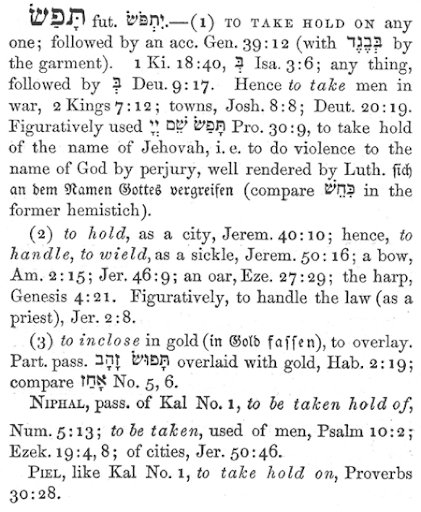
\includegraphics[width=10cm]{taphas}
Strong’s seems to imply it could be about manipulation:

 \begin{hebrew} תּפשׂ  \end{hebrew}

tâphaś 

taw-fas' 

A primitive root; to manipulate, that is, seize; chiefly to capture, wield; specifically to overlay; figuratively to use unwarrantably

KJV Usage: catch, handle, (lay, take) hold (on, over), stop, X surely, surprise, take.


As does Brown-Driver-Briggs' Hebrew Definitions (wield, use skillfully)


Mary Anna Bader writes in response to Lyn Bechtel the next:

	 	 	

I do not find "taphas" to be used in contexts describing mutual consensual relations anywhere in the Hebrew Bible. Let us consider those passages. When the verb "taphas" is used in Genesis 39:12, Potiphar's wife seized or caught hold of Joseph by his garment as she begged him to lie with her. Anything but mutuality is described here. Bechtel's Point that this verb is indicative of mutuality can be substantially undermined. Potiphar's wife, we would say today, was sexually harassing Joseph. He was not willing to participate in a sexual liaison with the wife of his master. 2 Kins 7:12 uses the verb "taphas" when Elisha described the ploy the Arameans had prepared, capturing the Israelites alive and then infiltrating the city. 
\url{https://www.answering-christianity.com/karim/Karim_-_articles_islamic_answers_-_part_3/Biblical%20Laws%20on%20Rape%20-%20commentary%20Deuter%2022_%2028-29.doc}


Contrary to Mary Anna Bader there is at least one exception to the non-mutuality in Eze 29:7


\section{Two Levels of Consent}
Two levels of consent required for marriage: 1 woman, 2 woman’s guardian

\subsection{Woman's Consent Was Required}

1. woman’s consent was required because of the laws against capturing and holding people as slaves. If you couldn’t capture people and you couldn’t hold them then you could force them to marry or have sex with you:

 “He who kidnaps a man and sells him, or if he is found in his hand, shall surely be put to death.(Ex 21:16)


21 “You shall neither mistreat a stranger nor oppress him, for you were strangers in the land of Egypt.
22 “You shall not afflict any widow or fatherless child. 23 If you afflict them in any way, and they cry at all to Me, I will surely hear their cry; 24 and My wrath will become hot, and I will kill you with the sword; your wives shall be widows, and your children fatherless. (Ex 22)


“Also you shall not oppress a stranger, for you know the heart of a stranger, because you were strangers in the land of Egypt. (Ex 23)


15 “You shall not give back to his master the slave who has escaped from his master to you. 16 He may dwell with you in your midst, in the place which he chooses within one of your gates, where it seems best to him; you shall not oppress him. (Deut 23)



\subsection{Father's Consent Was Required}

Women in their father’s house couldn’t consent without their father: 
 

Father’s are responsible for their daughter’s sexual and marital behavior:
‘Do not prostitute your daughter, to cause her to be a harlot, lest the land fall into harlotry, and the land become full of wickedness. (Lev 19:23)


“Nor shall you make marriages with them. You shall not give your daughter to their son, nor take their daughter for your son.”
(Deuteronomy 7:3)


That’s why they had to make a law specifically for the situation when the guardians were dead:


10 “When you go out to war against your enemies, and the Lord your God delivers them into your hand, and you take them captive, 11 and you see among the captives a beautiful woman, and desire her and would take her for your wife, 12 then you shall bring her home to your house, and she shall shave her head and trim her nails. 13 She shall put off the clothes of her captivity, remain in your house, and mourn her father and her mother a full month; after that you may go in to her and be her husband, and she shall be your wife. 14 And it shall be, if you have no delight in her, then you shall set her free, but you certainly shall not sell her for money; you shall not treat her brutally, because you have humbled her. (Deut 21)



1 Then Moses spoke to the heads of the tribes concerning the children of Israel, saying, “This is the thing which the Lord has commanded: 2 If a man makes a vow to the Lord, or swears an oath to bind himself by some agreement, he shall not break his word; he shall do according to all that proceeds out of his mouth.
3 “Or if a woman makes a vow to the Lord, and binds herself by some agreement while in her father’s house in her youth, 4 and her father hears her vow and the agreement by which she has bound herself, and her father holds his peace, then all her vows shall stand, and every agreement with which she has bound herself shall stand. 5 But if her father overrules her on the day that he hears, then none of her vows nor her agreements by which she has bound herself shall stand; and the Lord will release her, because her father overruled her.
6 “If indeed she takes a husband, while bound by her vows or by a rash utterance from her lips by which she bound herself, 7 and her husband hears it, and makes no response to her on the day that he hears, then her vows shall stand, and her agreements by which she bound herself shall stand. 8 But if her husband overrules her on the day that he hears it, he shall make void her vow which she took and what she uttered with her lips, by which she bound herself, and the Lord will release her.
9 “Also any vow of a widow or a divorced woman, by which she has bound herself, shall stand against her.
10 “If she vowed in her husband’s house, or bound herself by an agreement with an oath, 11 and her husband heard it, and made no response to her and did not overrule her, then all her vows shall stand, and every agreement by which she bound herself shall stand. 12 But if her husband truly made them void on the day he heard them, then whatever proceeded from her lips concerning her vows or concerning the agreement binding her, it shall not stand; her husband has made them void, and the Lord will release her. 13 Every vow and every binding oath to afflict her soul, her husband may confirm it, or her husband may make it void. 14 Now if her husband makes no response whatever to her from day to day, then he confirms all her vows or all the agreements that bind her; he confirms them, because he made no response to her on the day that he heard them. 15 But if he does make them void after he has heard them, then he shall bear her guilt.” (Numbers 30)

The state the woman was in in relation to her guardian changes the severity of the crime committed (compare to Deut 22:22-24:

20 ‘Whoever lies carnally with a woman who is betrothed to a man as a concubine, and who has not at all been redeemed nor given her freedom, for this there shall be scourging; but they shall not be put to death, because she was not free. 21 And he shall bring his trespass offering to the Lord, to the door of the tabernacle of meeting, a ram as a trespass offering. 22 The priest shall make atonement for him with the ram of the trespass offering before the Lord for his sin which he has committed. And the sin which he has committed shall be forgiven him. (Lev 19)

Philo compares seduction to rape seeming to imply it is not consensual because the father was not consulted:

XI. (64) But if any one should offer violence to a widow after her husband is dead, or after she has been otherwise divorced from him, and defile her, committing a lighter offence than adultery, and one that may perhaps be about half as serious, he shall not indeed be liable to the punishment of death, but he shall be impeached for violence, and insolence, and intemperance, having thus adopted the most infamous conduct as if it had been the most creditable; and the tribunal of the judge shall decide and condemn him to the penalty that he deserves to suffer. (65) Again, seduction is an offence which is similar and nearly related to adultery, as they are both sprung from one common mother, incontinence. But some of those persons who are accustomed to dignify shameful actions by specious names, call this love, blushing to confess the real truth concerning its character. But, nevertheless, though it may be akin to it, it is not in every respect similar to it, because it is an offence that does not spread so as to affect many families, as is the case with adultery, but it is limited to one house alone, that of the virgin who has been seduced. (66) Therefore we must say to a man who desires to enjoy a virgin who is a free-born citizen, "My good man, rejecting your shameless rashness and audacity, the sources of treachery and faithlessness, and all such feelings, do not allow yourself to be discovered to be wicked, either openly or secretly, (67) but if, indeed, you have any legitimate feeling of love for the maiden in your soul, go to her parents, if they are alive, and if they are not, then go to her brother or to her guardians, or to any other persons who chance to be her protectors, and having discovered to them your feelings towards her, as a free-born man should do, ask her in marriage, and implore them not to account you unworthy. (68) "For no one of those who have the guardianship of the maiden entrusted them could be so base as to oppose an earnest and persevering entreaty, and especially as to refuse you since you, would be found, by strict examination, not to have falsely pretended a passion which you do not feel, or to have conceived only a superficial love for her, but one which is genuine and thoroughly Established."\{4\}\{\#de 22:13.\} (69) But if any one, being insane and frantic, repudiating and discarding all the suggestions of reason, were to submit himself wholly to passion and desire as his masters, and looking, as people say, on might as stronger than right, were to ravish and seduce women, treating free-born women as slaves, and doing acts of war in time of peace, let such a man be led before the judges. (70) And if the damsel who has been forced has a father, let him take counsel and deal with the ravisher about espousing her; then if he refuse to do so, he shall give the damsel a dowry for another husband, being fined in a sum of money sufficient for this purpose. But if he consents and registers her as his wife, let him marry her at once without any delay, confessing a second time that he owes her the same dowry, and let him have no permission to delay or evade the fulfilment of this marriage; both because of his own conduct, in order that the mishap which took place respecting her first connection with a man may be comforted by a firm marriage, which nothing shall ever separate but death. (71) But if the damsel be an orphan and have no father, then let her be asked by the judges whether she is willing to take this man for her husband or not; and whether she agrees to do so or whether she refuses, still let her have the same dowry that the man would have agreed to give her while her father was yet alive.
(Philo)

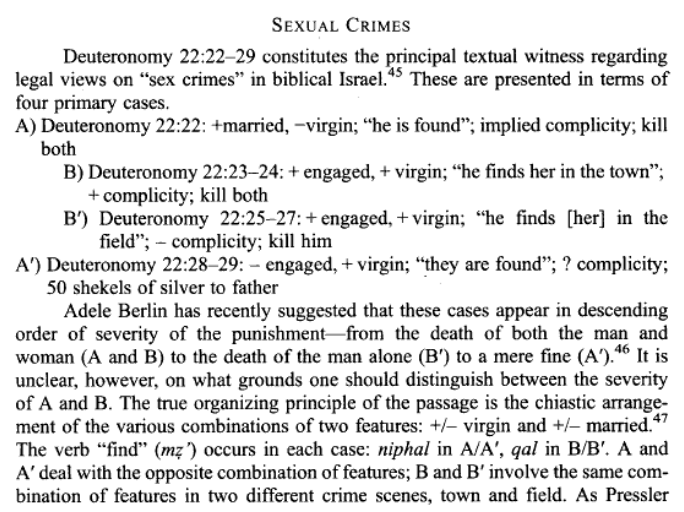
\includegraphics[width=10cm]{deuteronomy22_case_options}

This word is used in Deut 22:23,25,28 to imply these women were under someone’s authority. \url{https://studybible.info/search-interlinear/strongs/3816/start/90} however this word is not used in Deuteronomy 22:22 implying the situation there is something woman is expected to be fully responsible unlike in 28.



\begin{greek} παῖς, παιδός+ N3M/F 126-184-39-47-74=470
Gn 9,25.26.27; 12,16; 14,15
child (in relation to parents) Prv 29,15; slave, servant Gn 9,25; courtier, attendant 1 Sm 22,17; servant
(of humans in relation to God) Is 41,8; girl, young lady Gn 24,28; girl, slave, maid Ru 2,6; παῖδες
children Prv 4,1
ἐκ παιδός from childhood, from youth Gn 46,34
*Gn 26,18 οἱ παῖδες the servants-עבדי) Sam. Pent.) for MT בימי in the days of; *Gn 47,21 εἰς παῖδας for \end{greek}
servants\begin{hebrew} -עבדים/ל for MT ערים/ל into \end{hebrew} the cities; *Jos 7,7 \begin{greek} διεβίβασεν ὁ παῖς σου \end{greek} your servant brought over
\begin{hebrew}
 עבדך
העביר for MT העביר העברת you surely brought over; 
 \end{hebrew}
\begin{greek}  *Jer 47(40),9 τῶν παίδων of the servants of \end{greek}
\begin{hebrew}
  מעבדי
for MT עבוד/מ 
\end{hebrew}
\begin{greek}
from serving, see also 2 Kgs 25,24; *Prv 1,4 παιδὶ δὲ νέῳ but to a young child, but to
a little child double transl. of MT
\end{greek}
\begin{hebrew}
 נער young man
\end{hebrew}
Cf. AMUSIN 1986 132-136.145-146; DANIEL, S. 1966 103.104; HARL 1986a, 68.143.200; HEINEN 1984,
1287-1295; KATZ 1956, 268-269; LARCHER 1983, 245-246; LE BOULLUEC 1989, 109; SCHOLL 1983 7-
8.15; SPICQ 1978b, 220-224; STANTON 1988, 475-476; WEVERS 1990 46; 1993 319.567; 1995 173.357;
→NIDNTT; TWNT 

\url{http://www.glasovipisma.pbf.rs/phocadownload/knjige/greek%20lexicon%20for%20the%20septuagint.pdf}



Virgin word usage https://studybible.info/search-interlinear/strongs/3933

 Deuteronomy 22:23, 28 are the only ones that have this word in the 22:22-30 section

\begin{greek}
παρθένος,-ου+ \end{greek} N2F 16-10-17-12-12=67
Gn 24,14.16(bis).43.55
virgin Jgs 19,24; virgin (as adj.) Lv 21,3; young woman Ez 9,6; a girl of marriage-able age Gn 24,14
Cf. DODD 1976, 301-305; DOGNIEZ 1992, 257; DUBARLE 1978, 370-371; FORD 1966, 293-299; GESE
1971, 88; HARL 1986a, 200; HORSLEY 1987, 222-226; SEELIGMAN 1948 118-119(Is 7,14); SPICQ 1982,
519-521; WEGNER 1992, 112-113; →NIDNTT; TWNT



\section{This is not force}

 if this is non-consensual it is because the daughter cannot fully consent without her father
\subsection{Different situation}
that belongs with Deut 22:30 the context is the same as Deut 22:22

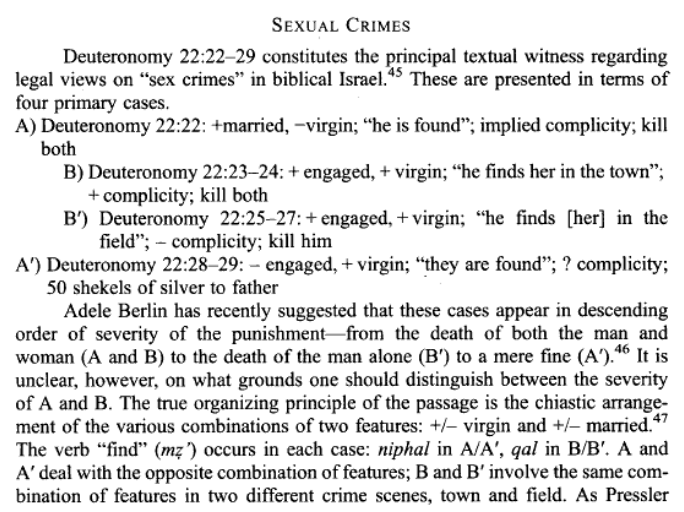
\includegraphics[width=10cm]{sexual_crimes}


1 It says right after “you shall not take your father’s wife” so it continues the theme of the rights of fathers after it started in Deuteronomy 22:28 (switched there from the rights of husbands)

2 it uses a different word

3 The word “taphas” can mean “take” as in taking a city or taking men in battle this is why it is the rights of fathers which continues in Deut 22:30 because he is “taking” her from her father.

4 Complicity is implied like in 22:22. No longer is it stated whether the woman cried out or whether she was in the city or the countryside which would leave the complicity implied like in Deuteronomy 22:22 since the woman now has to marry the person she slept with as does the man.

5 If we are to say this is rape since “taphas” is associated with war then we must say Deut 21:10-14 means rape as well since there is no information given about the woman’s consent.

6 There is the possibility of mutuality with taphas: “When they took hold H8610 of thee by thy hand, thou didst break, and rend all their shoulder: and when they leaned upon thee, thou brakest, and madest all their loins to be at a stand.” Eze 29:7

7 If taphas has the implication of taking people in war then I would argue that for the israelites this did not imply rape since the Israelites did not do this in war (as is also testified in Deu 21) so therefore consent is implied. The implication of “war” just refers to not consulting the father like in Deuteronomy 21:10-14 Also Philo connects seduction to acts of war.

\subsection{Word Difference}

In Deu 22:24 word for “humbled” is the same (Piel form) which does not mean rape.

Taphas means “to hold” while “chazaq” means “to hold fast.” Taphas does not have the context of force unlike chazaq which means to “bind tightly” or “be strong” or “overpower.” I think the reason why they didn’t use “laqach” is because it could be mistaken for “taking a wife” properly without more context given.  


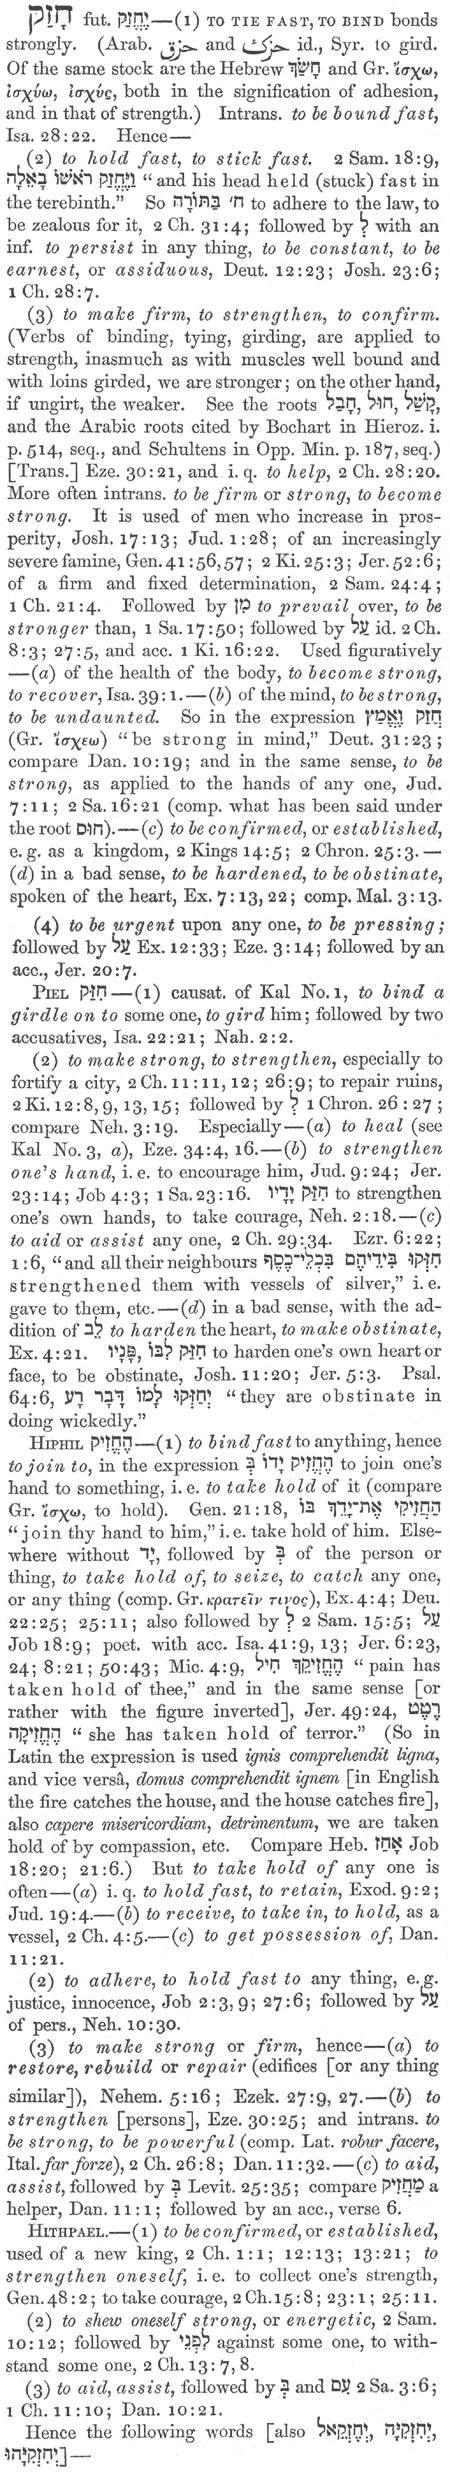
\includegraphics[width=4cm]{chazak}

\subsection{Word Definition Must Rely on Context}
\subsection{May be a mistake to rely on words, instead rely on context. Even “chazdaq” can be used non violently or violently in the same word form}


Stem: Hiphil
Aspect: Imperfect

Jdg 19:4
And his father in law, the damsel's father, retained H2388 him; and he abode with him three days: so they did eat and drink, and lodged there.



Stem: Hiphil
Aspect: Imperfect

2Ki 4:8
And it fell on a day, that Elisha passed to Shunem, where was a great woman; and she constrained H2388 him to eat bread. And so it was, that as oft as he passed by, he turned in thither to eat bread.



Stem: Hiphil
Aspect: Perfect

Deu 22:25
But if a man find a betrothed damsel in the field, and the man force H2388 her, and lie with her: then the man only that lay with her shall die:


Stem: Hiphil
Aspect: Imperfect
2Sa 13:11
And when she had brought them unto him to eat, he took hold H2388 of her, and said unto her, Come lie with me, my sister.

Stem: Qal
Aspect: Imperfect
2Sa 13:14
Howbeit he would not hearken unto her voice: but, being stronger H2388 than she, forced her, and lay with her.




Taphas (qal imperfect) to hold onto his brother while pleading with him:
Isa 3:6
When a man shall take hold h8610 of his brother of the house of his father, saying, Thou hast clothing, be thou our ruler, and let this ruin be under thy hand:
7 In that day he will protest, saying,
“I cannot cure your ills,
For in my house is neither food nor clothing;
Do not make me a ruler of the people.”


The crime is not connected to force but to humbling as in Deut 21:15 where she has no guardian:

Deu 22:22
If a man be found lying H7901 with a woman married to an husband, then they shall both of them die, both the man that lay H7901 with the woman, and the woman: so shalt thou put away evil from Israel.

Deu 22:29
Then the man that lay H7901 with her shall give unto the damsel's father fifty shekels of silver, and she shall be his wife; because he hath humbled her, he may not put her away all his days.



Gen 34:2
And when Shechem the son of Hamor the Hivite, prince of the country, saw her, he took her, and lay with her, and defiled her. H6031


Deu 21:14
And it shall be, if thou have no delight in her, then thou shalt let her go whither she will; but thou shalt not sell her at all for money, thou shalt not make merchandise of her, because thou hast humbled H6031 her.


Deu 22:24
Then ye shall bring them both out unto the gate of that city, and ye shall stone them with stones that they die; the damsel, because she cried not, being in the city; and the man, because he hath humbled H6031 his neighbour's wife: [but she was betrothed not married] so thou shalt put away evil from among you.


Deu 22:29
Then the man that lay with her shall give unto the damsel's father fifty shekels of silver, and she shall be his wife; because he hath humbled H6031 her, he may not put her away all his days.


Lam 5:11
They ravished H6031 the women in Zion, and the maids in the cities of Judah.


Eze 22:10
In thee have they discovered their fathers' nakedness: in thee have they humbled H6031 her that was set apart for pollution.


Eze 22:11
And one hath committed abomination with his neighbour's wife; and another hath lewdly defiled his daughter in law; and another in thee hath humbled H6031 his sister, his father's daughter.





Oddly enough the word for “force” that can mean rape is used for him forcing his concubine and for his father forcing him to stay there:

Jdg 19:4
And his father in law, the damsel's father, retained H2388 him; and he abode with him three days: so they did eat and drink, and lodged there.


Jdg 19:25
But the men would not hearken to him: so the man took H2388 his concubine, and brought her forth unto them; and they knew her, and abused her all the night until the morning: and when the day began to spring, they let her go.




Also of the concubine:

Jdg 19:25
But the men would not hearken to him: so the man took his concubine, and brought her forth unto them; and they knew her, and abused H5953 her all the night until the morning: and when the day began to spring, they let her go.





Judges uses completely different words when they took themselves wives by force:



Jdg 21:21
And see, and, behold, if the daughters of Shiloh come out to dance in dances, then come ye out of the vineyards, and catch H2414 you every man his wife of the daughters of Shiloh, and go to the land of Benjamin.


Jdg 21:23
And the children of Benjamin did so, and took h5375 them wives, according to their number, of them that danced, whom they caught: h1497 and they went and returned unto their inheritance, and repaired the cities, and dwelt in them.


Same with Samuel:


2Sa 13:11

And when she had brought them unto him to eat, he took hold H2388 of her, and said unto her, Come lie with me, my sister.

2Sa 13:14

Howbeit he would not hearken unto her voice: but, being stronger H2388 than she, forced her, and lay with her.



\subsection{The pre-mishnaic tradition which is older than the talmud agrees it is connected with Ex 22:16-17}

Exodus 22:16-17 implies that it is the right thing for them to marry “if her father absolutely refuses”, “he doth certainly endow her to himself for a wife” this is not something you would want legally in a case of rape.



None of the words the Temple scroll uses mean rape, only one of the words Josephus uses could be interpreted as rape and do not mean that in the LXX. Both of the stronger words philo uses could mean rape but also have other meanings in the LXX and the word “Biazo” he uses seems to have the woman as the direct object which has a pattern of making it “urging” rather than force: https://studybible.info/search-interlinear/strongs/G971 The word translated “ravish” could mean also mean “to snatch away or to carry off” implying try to take her sexually without compensating her father which leads me to my next point:


Conclusion: Josephus, Dead sea scrolls and Philo consider this to be seduction (at least partially) and put the two laws together

Either we are left with the idea that this primitive culture didn’t have a concept of what rape was and considered it was the same as seduction or we have to distinguish the two. Deut 22:26 suggests they did have this concept and it was strong enough to compare to murder. Also if we don’t distinguish rape and seduction we are left with the idea of that the woman is culpable in this situation. Since the rapist is not punished for his use of force we either must conclude that the woman got what she deserved by leaving home unprotected or we have to say that the Bible does not punish rape. Since Josphus, Philo and maybe even the people who wrote the dead sea scrolls had the septuagint they would have known that the same word “Biazo” is used in Deut 22:28 and Deut 22:25 and this would mean that they must have seen those words differently because they are used differently. You can reasonably combine the two laws together with my view: that this was rape but not forcible rape rather rape due to lack of consent of the father hence it is identical with seduction in Exodus 22:15-16 and can be combined, otherwise, again we are left with a problem of bible that doesn’t care about forcible rape. 

\subsection{Lastly the words used for “taking” a wife and “finding” a woman can be used in violent contexts however like “taphas” context is key to decide whether they are violent:}

Laqach can be associated with violence but it is not always used that way, the Qal perfect form:

 Deu 22:14

And give occasions of speech against her, and bring up an evil name upon her, and say, I took H3947 this woman, and when I came to her, I found her not a maid:


 Deu 22:18

And the elders of that city shall take H3947 that man and chastise him;


 Jos 7:24

And Joshua, and all Israel with him, took H3947Achan the son of Zerah, and the silver, and the garment, and the wedge of gold, and his sons, and his daughters, and his oxen, and his asses, and his sheep, and his tent, and all that he had: and they brought them unto the valley of Achor.


 Jos 11:19

There was not a city that made peace with the children of Israel, save the Hivites the inhabitants of Gibeon: all other they took H3947 in battle.



The word for “found” H4672 can even be used in associating with a violent act:

Deu 31:17
Then my anger shall be kindled against them in that day, and I will forsake them, and I will hide my face from them, and they shall be devoured, and many evils and troubles shall befall H4672 them; so that they will say in that day, Are not these evils come H4672 upon us, because our God is not among us?


\section{Things left to decide:}

Richard Abbot writes in his  footnote on Deut. 22:28 the next about the Hebrew word "taphas": 

tâphas, here used in the Qal perfect form with suffix, has a violent or forceful air, hence seize. 2

\section{appendix, Philo, Josephus}


XI. (64) But if any one should offer violence to a widow after her husband is dead, or after she has been otherwise divorced from him, and defile her, committing a lighter offence than adultery, and one that may perhaps be about half as serious, he shall not indeed be liable to the punishment of death, but he shall be impeached for violence, and insolence, and intemperance, having thus adopted the most infamous conduct as if it had been the most creditable; and the tribunal of the judge shall decide and condemn him to the penalty that he deserves to suffer. (65) Again, seduction is an offence which is similar and nearly related to adultery, as they are both sprung from one common mother, incontinence. But some of those persons who are accustomed to dignify shameful actions by specious names, call this love, blushing to confess the real truth concerning its character. But, nevertheless, though it may be akin to it, it is not in every respect similar to it, because it is an offence that does not spread so as to affect many families, as is the case with adultery, but it is limited to one house alone, that of the virgin who has been seduced. (66) Therefore we must say to a man who desires to enjoy a virgin who is a free-born citizen, "My good man, rejecting your shameless rashness and audacity, the sources of treachery and faithlessness, and all such feelings, do not allow yourself to be discovered to be wicked, either openly or secretly, (67) but if, indeed, you have any legitimate feeling of love for the maiden in your soul, go to her parents, if they are alive, and if they are not, then go to her brother or to her guardians, or to any other persons who chance to be her protectors, and having discovered to them your feelings towards her, as a free-born man should do, ask her in marriage, and implore them not to account you unworthy. (68) "For no one of those who have the guardianship of the maiden entrusted them could be so base as to oppose an earnest and persevering entreaty, and especially as to refuse you since you, would be found, by strict examination, not to have falsely pretended a passion which you do not feel, or to have conceived only a superficial love for her, but one which is genuine and thoroughly Established."\{4\}\{\#de 22:13.\} (69) But if any one, being insane and frantic, repudiating and discarding all the suggestions of reason, were to submit himself wholly to passion and desire as his masters, and looking, as people say, on might as stronger than right, were to ravish and seduce women, treating free-born women as slaves, and doing acts of war in time of peace, let such a man be led before the judges. (70) And if the damsel who has been forced has a father, let him take counsel and deal with the ravisher about espousing her; then if he refuse to do so, he shall give the damsel a dowry for another husband, being fined in a sum of money sufficient for this purpose. But if he consents and registers her as his wife, let him marry her at once without any delay, confessing a second time that he owes her the same dowry, and let him have no permission to delay or evade the fulfilment of this marriage; both because of his own conduct, in order that the mishap which took place respecting her first connection with a man may be comforted by a firm marriage, which nothing shall ever separate but death. (71) But if the damsel be an orphan and have no father, then let her be asked by the judges whether she is willing to take this man for her husband or not; and whether she agrees to do so or whether she refuses, still let her have the same dowry that the man would have agreed to give her while her father was yet alive.

\url{http://www.earlyjewishwritings.com/text/philo/book29.html}


\begin{greek} ἁρπάζω+ V 4-4-17-11-5=41
Gn 37,33; Lv 5,23; 19,13; Dt 28,31; Jgs 21,21
to snatch away [τι ἔκ τινος] 2 Sm 23,21; to carry off [τινα] Gn 37,33; to seize [τινα] Jgs 21,21; to
captivate, to ravish [τι] Jdt 16,9
→ NIDNTT; TWNT
(→ἀν-, δι-, ἐξ-, συν-) 
\end{greek}

\begin{greek}
βιάζομαι+ V 4-6-0-1-6=17
Gn 33,11; Ex 19,24; Dt 22,25.28; JgsA 13,15
to urge, to insist, to constrain [τινα] Gn 33,11; to force [τινα] Ex 19,24; to lay hands upon, violate [τινα]
Est 7,8; to break violently into [τι] 2 Mc 14,41; to constrain to [+inf.] Ex 19,24
Cf. HELBING 1928, 13; SPICQ 1978a, 189-194; →TWNT
(→ἀπο-, δια-, ἐκ-, κατα-, παρα-) 
\end{greek}


If any one has been espoused to a woman as to a virgin, and does not afterward find her so to be, let him bring his action, and accuse her, and let him make use of such indications 1 to prove his accusation as he is furnished withal; and let the father or the brother of the damsel, or some one that is after them nearest of kin to her, defend her If the damsel obtain a sentence in her favor, that she had not been guilty, let her live with her husband that accused her; and let him not have any further power at all to put her away, unless she give him very great occasions of suspicion, and such as can be no way contradicted. But for him that brings an accusation and calumny against his wife in an impudent and rash manner, let him be punished by receiving forty stripes save one, and let him pay fifty shekels to her father: but if the damsel be convicted, as having been corrupted, and is one of the common people, let her be stoned, because she did not preserve her virginity till she were lawfully married; but if she were the daughter of a priest, let her be burnt alive. If any one has two wives, and if he greatly respect and be kind to one of them, either out of his affection to her, or for her beauty, or for some other reason, while the other is of less esteem with him; and if the son of her that is beloved be the younger by birth than another born of the other wife, but endeavors to obtain the right of primogeniture from his father's kindness to his mother, and would thereby obtain a double portion of his father's substance, for that double portion is what I have allotted him in the laws, - let not this be permitted; for it is unjust that he who is the elder by birth should be deprived of what is due to him, on the father's disposition of his estate, because his mother was not equally regarded by him. He that hath corrupted a damsel espoused to another man, in case he had her consent, let both him and her be put to death, for they are both equally guilty; the man, because he persuaded the woman willingly to submit to a most impure action, and to prefer it to lawful wedlock; the woman, because she was persuaded to yield herself to be corrupted, either for pleasure or for gain. However, if a man light on a woman when she is alone, and forces her, where nobody was present to come to her assistance, let him only be put to death. Let him that hath corrupted a virgin not yet espoused marry her; but if the father of the damsel be not willing that she should be his wife, let him pay fifty shekels as the price of her prostitution.

josephus:

\url{http://www.perseus.tufts.edu/hopper/text?doc=Perseus%3Atext%3A1999.01.0145%3Abook%3D4%3Awhiston+chapter%3D8%3Awhiston+section%3D23}

josephus in greek:

\url{http://www.perseus.tufts.edu/hopper/text?doc=Perseus%3Atext%3A1999.01.0146%3Abook%3D4%3Awhiston+chapter%3D8%3Awhiston+section%3D23}

The two words in red he uses in LSJ:

\url{http://www.perseus.tufts.edu/hopper/morph?l=u%28%2Fbrews&la=greek&can=u%28%2Fbrews0&prior=th=s#lexicon}

\url{http://www.perseus.tufts.edu/hopper/morph?l=fqei%2Fras&la=greek&can=fqei%2Fras1&prior=o(#lexicon}


Only one of those two words (in red) can mean rape and it doesn't seem to mean that in the septuagint lexicon:


The word he uses in the septuagint context and lexicons: \url{https://studybible.info/search-interlinear/strongs/5196}


ὕβρις,-εως+ N3F 1-0-32-16-13=62 Lv 26,19; Is 9,8; 10,33; 13,11(bis) insolence, pride, arrogance Est 4,17d; shame, insult, mistreatment Sir 10,8; hardship 3 Mc 3,25 ἡ ὕβρις τῆς ἰσχύος αὐτῆς hybris, i.e. haughty behaviour, (on account) of her strength Ez 33,28 *Mi 6,10 ὕβρεως (of) pride-זדון for MT רזון emaciation; *Prv 14,10 ὕβρει (with) pride-זד for MT זר stranger Cf. BERTRAM 1964, 29-38; →NIDNTT; TWNT 

http://www.glasovipisma.pbf.rs/phocadownload/knjige/greek%20lexicon%20for%20the%20septuagint.pdf


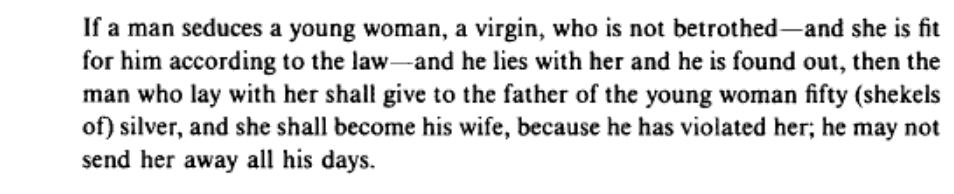
\includegraphics[width=4cm]{dead_sea_scrolls}

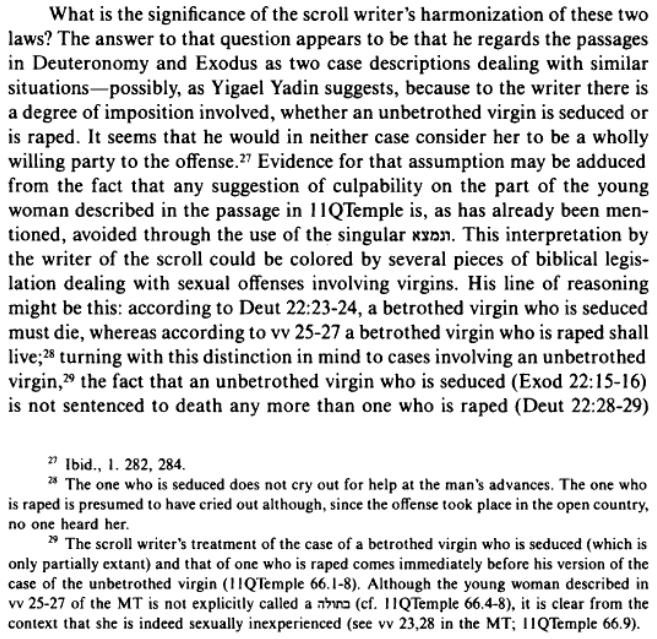
\includegraphics[width=4cm]{dss_comment}

G Dinah 
  εκοιμήθη in Genesis 30:16 (going to bed in story of the mandrakes) is the same as in Gen 34:2 


Luke 20:29 V-APA-NMS
\begin{greek}
GRK: ὁ πρῶτος λαβὼν γυναῖκα ἀπέθανεν
\end{greek}
NAS: and the first took a wife


Deuteronomy 22:22 root word for “humbled” is the same in Gen 34:2

 https://studybible.info/interlinear/Deuteronomy%2022:22



 Deu 22:24 word for “humbled” is the same in Gen 34:2 (in the Piel form)


Gen 30:15 word for “sleep with” is the same in Gen 34:2 (in the Qal form)

Then ye shall bring them both out unto the gate of that city, and ye shall stone them with stones that they die; the damsel, because she cried not, being in the city; and the man, because he hath humbled H6031 his neighbour's wife: so thou shalt put away evil from among you.


Greek words translated from the qal perfect “taphas” to find what is common between all:
4815

Deu 21:19, Jos 8:23, 2 Kings 14:7, 2 Kings 14:13
\begin{greek}
συλλαμβάνω+ V 23-28-25-15-27=118
Gn 4,1.17.25; 16,4; 19,36
A: to lay hold of, to arrest [τινα] (of pers.) 1 Kgs 13,4; to take, to catch [τινα] (of anim.) Jgs 15,4; to
take, to capture [τι] 2 Kgs 14,7; to conceive [abs.] Gn 4,1; id. [τινα] Ct 3,4; id. [τι] (metaph.) Ps 7,15
P: to be taken (from earth) Jb 22,16
συλλήμψεται μεθ᾽ ἑαυτοῦ he shall take with himself Ex 12,4
*Ct 8,2 τῆς συλλαβούσης με of her who conceived me-◊ילד for MT ◊למד she teaches me?, cpr. Ct 3,4
 (הורתי)
Cf. HELBING 1928, 310; MARGOLIS, M. 1906a=1972 78-79; →NIDNTT; TWNT
\end{greek}


2638

2 Chronicles 25:23
\begin{greek}
καταλαμβάνω+ V 13-31-19-20-43=126
Gn 19,19; 31,23.25; 44,4; Ex 15,9
A: to take, lay hold of [τι] Jgs 7,24; to take, to overtake [τινα] (of God) Jb 5,13; to overtake, to befall
[τινα] (of evil) Gn 19,19; to overtake [τινα] (often after a pursuit) Gn 31,23; to reach [τινα] (of men
reaching God) Mi 6,6; to overtake, to take hold of [τινα] (of sin; metaph.) Ps 39(40),13; to lay hold of, to
come over, to overtake [τινα] (of feelings; metaph.) Ps 68(69),25; to take prisoner [τινα] 2 Chr 25,23; to
take, to capture [τι] (of city) 2 Sm 12,26
to comprehend, to understand [τι] Jb 34,24, cpr. DnLXX 1,20
to find sb doing [τινα +pred.] 1 Ezr 6,8; to detect, to catch in the act of doing (esp. of the detection of
adultery) [τινα] SusLXX 58, see also Jer 3,8 (double transl. of the Hebr.)
M: to seize, to lay hold on [τι] Prv 1,13; to overtake, to take hold of [τινα] (of sin) Jdt 11,11; to take, to
capture [τι] (of city) Nm 21,32; to occupy, to keep [τι] 1 Mc 11,46
P: to be taken, to be stolen Ex 22,3; to be apprehended, to be taken hold of Prv 2,19; to be detected Ob 6;
to be convicted Jer 3,8
κατέλαβον τὸν Μανασση ἐν δεσμοῖς they took Manasseh in bonds, they captured Manasseh 2 Chr 33,11;
τοῦ φιλίαν καταλαβέσθαι τοῖς Ιουδαίοις to form friendship with the Jews 1 Mc 10,23; καταλάβωσιν
τρίβους εὐθείας they comprehend, they understand the paths of life Prv 2,19; κατειλημμένη ἐν ἀγῶνι
θανάτου seized by the agony of death Est 4,17k; καταλήμψεται ὁ ἀλοητὸς τὸν τρύγητον the
threshingtime shall over-take the vintage Lv 26,5; οἳ κατελάβοσαν τοὺς πατέρας ὑμῶν who convicted
your fathers Zech 1,6 
*2 Chr 9,20 χρυσίῳ κατειλημμένα with gold, stolen? corr.? χρυσίῳ κατακεκλεισμένα for MT סגור זהב
covered with gold, of pure gold, cpr. 1 Kgs 6,20; *Jer 28(51),34 κατέλαβέν με he came upon me-ישׂיגני ?
for MT יציגני he put me away
Cf. MARGOLIS, M. 1906a=1972 77; →LSJ Suppl (2 Chr 9,20) 
\end{greek}

2629.2

Jer 40:10
\begin{greek}
κατακόπτω+ V 3-6-10-1-2=22

κατακρατέω V 0-4-8-0-18=30
1 Sm 14,42; 1 Kgs 12,24u; 2 Chr 12,1.4; Jer 8,5
A: to prevail against [τινος] 1 Sm 14,42; to prevail [abs.] Mi 1,9; to become master of, to conquer
[τινος] 1 Mc 8,4; to obtain or retain possession of [τινος] 2 Chr 12,4; to usurp [τινος] 1 Mc 15,3; to
occupy [τι] Jer 47(40),10; to seize upon, to overcome [τινος] (of pains) Mi 4,9; to be master of, to rule
over [τι] 1 Ezr 4,2; to strengthen oneself (of pers.) 1 Kgs 12,24u; to strengthen, to make stronger [τινος]
Na 3,14
P: to strengthen oneself (of pers.) Jer 8,5; to grow strong (of things) 2 Chr 12,1; to be in possession of
[ὑπό τινος] 1 Mc 15,33
κατακρατεῖ τοῦ ἐννοήματος αὐτοῦ he controls his thoughts Sir 21,11 
\end{greek}

This one really is a fluke and shouldn’t belong in the list but I included it for completeness. It’s because taphas is translated “oath” because it translates “take the lord’s name in vain” to “swear an oath by the name of God”

Proverbs 30:9 
\begin{greek}
ὄμνυμι+
/ὀμνύω+ V 64-48-34-17-25=188
Gn 21,23.24.31; 22,16; 24,7
to swear Gn 21,24; to swear to sb [τινι] Gn 24,7; to swear sth to sb, to confirm sth for sb with an oath
[τινί τινα] Gn 21,23; id. [τινι κατά τινος] Ex 32,13; to swear to give [τί τινι] Gn 50,24; to swear by
[τινι] Dt 32,40; id. [κατά τινος] Gn 22,16; id. [ἔν τινι] Jgs 21,7; to swear to sb that [τινι +inf. fut.] Jdt
8,9; to swear that [+inf. pft.] Ex 22,7; to swear falsely [τι] Prv 30,9
οἱ ὀμνύμενοι them by whom they swear Wis 14,31; οὐκ ὤμοσεν ἐπὶ δόλῳ τῷ πλησίον αὐτοῦ nor did he
swear deceitfully to his neighbour Ps 23(24),4
*Ez 6,9 ὀμώμοκα I have sworn-נשׁבעתי◊ שׁבע for MT נשׁברתי◊ שׁבר I was broken, I was crushed
Cf. DORIVAL 1994, 514; HARL 1986a, 55; HELBING 1928, 71-72; LUST 1994 155-164(Dt 32,40); WEVERS
1993, 310; →NIDNTT; TWNT
(→ἐξ-) 
\end{greek}


Taphas

Stem: Qal 

Form: participle 

Gen 4:21
And his brother's name was Jubal: he was the father of all such as handle the harp and organ.
\begin{greek}
καταδείκνυμι V 1-0-4-0-0=5
Gn 4,21; Is 40,26; 41,20; 43,15; 45,18
to discover and make known, to invent [τι] Gn 4,21; to appoint, to create [τινα] Is 43,15; to create, to
fashion [τι] Is 45,18
Cf. RENEHAN 1975, 117; →LSJ Suppl; LSJ RSuppl 
\end{greek}



Stem: Qal
Aspect: Imperfect

Gen 39:12
And she caught him by his garment, saying, Lie with me: and he left his garment in her hand, and fled, and got him out.
\begin{greek}
ἐπισπάω+ V 1-0-2-0-8=11
Gn 39,12; Is 5,18; Na 3,14; Jdt 12,12; 1 Mc 14,1
M: to draw (in or to), to call (in)
Cf. LARCHER 1983, 196 
\end{greek}





Taphas

Perfect Qal form:

Deu 21:19
Then shall his father and his mother lay hold H8610 on him, and bring him out unto the elders of his city, and unto the gate of his place;



Jos 8:23
And the king of Ai they took H8610 alive, and brought him to Joshua.



2Ki 14:7
He slew of Edom in the valley of salt ten thousand, and took H8610 Selah by war, and called the name of it Joktheel unto this day.


2Ki 14:13
And Jehoash king of Israel took H8610 Amaziah king of Judah, the son of Jehoash the son of Ahaziah, at Bethshemesh, and came to Jerusalem, and brake down the wall of Jerusalem from the gate of Ephraim unto the corner gate, four hundred cubits.

2Ch 25:23

And Joash the king of Israel took H8610 Amaziah king of Judah, the son of Joash, the son of Jehoahaz, at Bethshemesh, and brought him to Jerusalem, and brake down the wall of Jerusalem from the gate of Ephraim to the corner gate, four hundred cubits.



Pro 30:9
Lest I be full, and deny thee, and say, Who is the LORD? or lest I be poor, and steal, and take H8610 the name of my God in vain.

Jer 40:10
As for me, behold, I will dwell at Mizpah to serve the Chaldeans, which will come unto us: but ye, gather ye wine, and summer fruits, and oil, and put them in your vessels, and dwell in your cities that ye have taken. H8610



\section{GNU Free Documentation License}

                GNU Free Documentation License
                 Version 1.3, 3 November 2008


 Copyright (C) 2000, 2001, 2002, 2007, 2008 Free Software Foundation, Inc.
     <https://fsf.org/>
 Everyone is permitted to copy and distribute verbatim copies
 of this license document, but changing it is not allowed.

0. PREAMBLE

The purpose of this License is to make a manual, textbook, or other
functional and useful document "free" in the sense of freedom: to
assure everyone the effective freedom to copy and redistribute it,
with or without modifying it, either commercially or noncommercially.
Secondarily, this License preserves for the author and publisher a way
to get credit for their work, while not being considered responsible
for modifications made by others.

This License is a kind of "copyleft", which means that derivative
works of the document must themselves be free in the same sense.  It
complements the GNU General Public License, which is a copyleft
license designed for free software.

We have designed this License in order to use it for manuals for free
software, because free software needs free documentation: a free
program should come with manuals providing the same freedoms that the
software does.  But this License is not limited to software manuals;
it can be used for any textual work, regardless of subject matter or
whether it is published as a printed book.  We recommend this License
principally for works whose purpose is instruction or reference.


1. APPLICABILITY AND DEFINITIONS

This License applies to any manual or other work, in any medium, that
contains a notice placed by the copyright holder saying it can be
distributed under the terms of this License.  Such a notice grants a
world-wide, royalty-free license, unlimited in duration, to use that
work under the conditions stated herein.  The "Document", below,
refers to any such manual or work.  Any member of the public is a
licensee, and is addressed as "you".  You accept the license if you
copy, modify or distribute the work in a way requiring permission
under copyright law.

A "Modified Version" of the Document means any work containing the
Document or a portion of it, either copied verbatim, or with
modifications and/or translated into another language.

A "Secondary Section" is a named appendix or a front-matter section of
the Document that deals exclusively with the relationship of the
publishers or authors of the Document to the Document's overall
subject (or to related matters) and contains nothing that could fall
directly within that overall subject.  (Thus, if the Document is in
part a textbook of mathematics, a Secondary Section may not explain
any mathematics.)  The relationship could be a matter of historical
connection with the subject or with related matters, or of legal,
commercial, philosophical, ethical or political position regarding
them.

The "Invariant Sections" are certain Secondary Sections whose titles
are designated, as being those of Invariant Sections, in the notice
that says that the Document is released under this License.  If a
section does not fit the above definition of Secondary then it is not
allowed to be designated as Invariant.  The Document may contain zero
Invariant Sections.  If the Document does not identify any Invariant
Sections then there are none.

The "Cover Texts" are certain short passages of text that are listed,
as Front-Cover Texts or Back-Cover Texts, in the notice that says that
the Document is released under this License.  A Front-Cover Text may
be at most 5 words, and a Back-Cover Text may be at most 25 words.

A "Transparent" copy of the Document means a machine-readable copy,
represented in a format whose specification is available to the
general public, that is suitable for revising the document
straightforwardly with generic text editors or (for images composed of
pixels) generic paint programs or (for drawings) some widely available
drawing editor, and that is suitable for input to text formatters or
for automatic translation to a variety of formats suitable for input
to text formatters.  A copy made in an otherwise Transparent file
format whose markup, or absence of markup, has been arranged to thwart
or discourage subsequent modification by readers is not Transparent.
An image format is not Transparent if used for any substantial amount
of text.  A copy that is not "Transparent" is called "Opaque".

Examples of suitable formats for Transparent copies include plain
ASCII without markup, Texinfo input format, LaTeX input format, SGML
or XML using a publicly available DTD, and standard-conforming simple
HTML, PostScript or PDF designed for human modification.  Examples of
transparent image formats include PNG, XCF and JPG.  Opaque formats
include proprietary formats that can be read and edited only by
proprietary word processors, SGML or XML for which the DTD and/or
processing tools are not generally available, and the
machine-generated HTML, PostScript or PDF produced by some word
processors for output purposes only.

The "Title Page" means, for a printed book, the title page itself,
plus such following pages as are needed to hold, legibly, the material
this License requires to appear in the title page.  For works in
formats which do not have any title page as such, "Title Page" means
the text near the most prominent appearance of the work's title,
preceding the beginning of the body of the text.

The "publisher" means any person or entity that distributes copies of
the Document to the public.

A section "Entitled XYZ" means a named subunit of the Document whose
title either is precisely XYZ or contains XYZ in parentheses following
text that translates XYZ in another language.  (Here XYZ stands for a
specific section name mentioned below, such as "Acknowledgements",
"Dedications", "Endorsements", or "History".)  To "Preserve the Title"
of such a section when you modify the Document means that it remains a
section "Entitled XYZ" according to this definition.

The Document may include Warranty Disclaimers next to the notice which
states that this License applies to the Document.  These Warranty
Disclaimers are considered to be included by reference in this
License, but only as regards disclaiming warranties: any other
implication that these Warranty Disclaimers may have is void and has
no effect on the meaning of this License.

2. VERBATIM COPYING

You may copy and distribute the Document in any medium, either
commercially or noncommercially, provided that this License, the
copyright notices, and the license notice saying this License applies
to the Document are reproduced in all copies, and that you add no
other conditions whatsoever to those of this License.  You may not use
technical measures to obstruct or control the reading or further
copying of the copies you make or distribute.  However, you may accept
compensation in exchange for copies.  If you distribute a large enough
number of copies you must also follow the conditions in section 3.

You may also lend copies, under the same conditions stated above, and
you may publicly display copies.


3. COPYING IN QUANTITY

If you publish printed copies (or copies in media that commonly have
printed covers) of the Document, numbering more than 100, and the
Document's license notice requires Cover Texts, you must enclose the
copies in covers that carry, clearly and legibly, all these Cover
Texts: Front-Cover Texts on the front cover, and Back-Cover Texts on
the back cover.  Both covers must also clearly and legibly identify
you as the publisher of these copies.  The front cover must present
the full title with all words of the title equally prominent and
visible.  You may add other material on the covers in addition.
Copying with changes limited to the covers, as long as they preserve
the title of the Document and satisfy these conditions, can be treated
as verbatim copying in other respects.

If the required texts for either cover are too voluminous to fit
legibly, you should put the first ones listed (as many as fit
reasonably) on the actual cover, and continue the rest onto adjacent
pages.

If you publish or distribute Opaque copies of the Document numbering
more than 100, you must either include a machine-readable Transparent
copy along with each Opaque copy, or state in or with each Opaque copy
a computer-network location from which the general network-using
public has access to download using public-standard network protocols
a complete Transparent copy of the Document, free of added material.
If you use the latter option, you must take reasonably prudent steps,
when you begin distribution of Opaque copies in quantity, to ensure
that this Transparent copy will remain thus accessible at the stated
location until at least one year after the last time you distribute an
Opaque copy (directly or through your agents or retailers) of that
edition to the public.

It is requested, but not required, that you contact the authors of the
Document well before redistributing any large number of copies, to
give them a chance to provide you with an updated version of the
Document.


4. MODIFICATIONS

You may copy and distribute a Modified Version of the Document under
the conditions of sections 2 and 3 above, provided that you release
the Modified Version under precisely this License, with the Modified
Version filling the role of the Document, thus licensing distribution
and modification of the Modified Version to whoever possesses a copy
of it.  In addition, you must do these things in the Modified Version:

A. Use in the Title Page (and on the covers, if any) a title distinct
   from that of the Document, and from those of previous versions
   (which should, if there were any, be listed in the History section
   of the Document).  You may use the same title as a previous version
   if the original publisher of that version gives permission.
B. List on the Title Page, as authors, one or more persons or entities
   responsible for authorship of the modifications in the Modified
   Version, together with at least five of the principal authors of the
   Document (all of its principal authors, if it has fewer than five),
   unless they release you from this requirement.
C. State on the Title page the name of the publisher of the
   Modified Version, as the publisher.
D. Preserve all the copyright notices of the Document.
E. Add an appropriate copyright notice for your modifications
   adjacent to the other copyright notices.
F. Include, immediately after the copyright notices, a license notice
   giving the public permission to use the Modified Version under the
   terms of this License, in the form shown in the Addendum below.
G. Preserve in that license notice the full lists of Invariant Sections
   and required Cover Texts given in the Document's license notice.
H. Include an unaltered copy of this License.
I. Preserve the section Entitled "History", Preserve its Title, and add
   to it an item stating at least the title, year, new authors, and
   publisher of the Modified Version as given on the Title Page.  If
   there is no section Entitled "History" in the Document, create one
   stating the title, year, authors, and publisher of the Document as
   given on its Title Page, then add an item describing the Modified
   Version as stated in the previous sentence.
J. Preserve the network location, if any, given in the Document for
   public access to a Transparent copy of the Document, and likewise
   the network locations given in the Document for previous versions
   it was based on.  These may be placed in the "History" section.
   You may omit a network location for a work that was published at
   least four years before the Document itself, or if the original
   publisher of the version it refers to gives permission.
K. For any section Entitled "Acknowledgements" or "Dedications",
   Preserve the Title of the section, and preserve in the section all
   the substance and tone of each of the contributor acknowledgements
   and/or dedications given therein.
L. Preserve all the Invariant Sections of the Document,
   unaltered in their text and in their titles.  Section numbers
   or the equivalent are not considered part of the section titles.
M. Delete any section Entitled "Endorsements".  Such a section
   may not be included in the Modified Version.
N. Do not retitle any existing section to be Entitled "Endorsements"
   or to conflict in title with any Invariant Section.
O. Preserve any Warranty Disclaimers.

If the Modified Version includes new front-matter sections or
appendices that qualify as Secondary Sections and contain no material
copied from the Document, you may at your option designate some or all
of these sections as invariant.  To do this, add their titles to the
list of Invariant Sections in the Modified Version's license notice.
These titles must be distinct from any other section titles.

You may add a section Entitled "Endorsements", provided it contains
nothing but endorsements of your Modified Version by various
parties--for example, statements of peer review or that the text has
been approved by an organization as the authoritative definition of a
standard.

You may add a passage of up to five words as a Front-Cover Text, and a
passage of up to 25 words as a Back-Cover Text, to the end of the list
of Cover Texts in the Modified Version.  Only one passage of
Front-Cover Text and one of Back-Cover Text may be added by (or
through arrangements made by) any one entity.  If the Document already
includes a cover text for the same cover, previously added by you or
by arrangement made by the same entity you are acting on behalf of,
you may not add another; but you may replace the old one, on explicit
permission from the previous publisher that added the old one.

The author(s) and publisher(s) of the Document do not by this License
give permission to use their names for publicity for or to assert or
imply endorsement of any Modified Version.


5. COMBINING DOCUMENTS

You may combine the Document with other documents released under this
License, under the terms defined in section 4 above for modified
versions, provided that you include in the combination all of the
Invariant Sections of all of the original documents, unmodified, and
list them all as Invariant Sections of your combined work in its
license notice, and that you preserve all their Warranty Disclaimers.

The combined work need only contain one copy of this License, and
multiple identical Invariant Sections may be replaced with a single
copy.  If there are multiple Invariant Sections with the same name but
different contents, make the title of each such section unique by
adding at the end of it, in parentheses, the name of the original
author or publisher of that section if known, or else a unique number.
Make the same adjustment to the section titles in the list of
Invariant Sections in the license notice of the combined work.

In the combination, you must combine any sections Entitled "History"
in the various original documents, forming one section Entitled
"History"; likewise combine any sections Entitled "Acknowledgements",
and any sections Entitled "Dedications".  You must delete all sections
Entitled "Endorsements".


6. COLLECTIONS OF DOCUMENTS

You may make a collection consisting of the Document and other
documents released under this License, and replace the individual
copies of this License in the various documents with a single copy
that is included in the collection, provided that you follow the rules
of this License for verbatim copying of each of the documents in all
other respects.

You may extract a single document from such a collection, and
distribute it individually under this License, provided you insert a
copy of this License into the extracted document, and follow this
License in all other respects regarding verbatim copying of that
document.


7. AGGREGATION WITH INDEPENDENT WORKS

A compilation of the Document or its derivatives with other separate
and independent documents or works, in or on a volume of a storage or
distribution medium, is called an "aggregate" if the copyright
resulting from the compilation is not used to limit the legal rights
of the compilation's users beyond what the individual works permit.
When the Document is included in an aggregate, this License does not
apply to the other works in the aggregate which are not themselves
derivative works of the Document.

If the Cover Text requirement of section 3 is applicable to these
copies of the Document, then if the Document is less than one half of
the entire aggregate, the Document's Cover Texts may be placed on
covers that bracket the Document within the aggregate, or the
electronic equivalent of covers if the Document is in electronic form.
Otherwise they must appear on printed covers that bracket the whole
aggregate.


8. TRANSLATION

Translation is considered a kind of modification, so you may
distribute translations of the Document under the terms of section 4.
Replacing Invariant Sections with translations requires special
permission from their copyright holders, but you may include
translations of some or all Invariant Sections in addition to the
original versions of these Invariant Sections.  You may include a
translation of this License, and all the license notices in the
Document, and any Warranty Disclaimers, provided that you also include
the original English version of this License and the original versions
of those notices and disclaimers.  In case of a disagreement between
the translation and the original version of this License or a notice
or disclaimer, the original version will prevail.

If a section in the Document is Entitled "Acknowledgements",
"Dedications", or "History", the requirement (section 4) to Preserve
its Title (section 1) will typically require changing the actual
title.


9. TERMINATION

You may not copy, modify, sublicense, or distribute the Document
except as expressly provided under this License.  Any attempt
otherwise to copy, modify, sublicense, or distribute it is void, and
will automatically terminate your rights under this License.

However, if you cease all violation of this License, then your license
from a particular copyright holder is reinstated (a) provisionally,
unless and until the copyright holder explicitly and finally
terminates your license, and (b) permanently, if the copyright holder
fails to notify you of the violation by some reasonable means prior to
60 days after the cessation.

Moreover, your license from a particular copyright holder is
reinstated permanently if the copyright holder notifies you of the
violation by some reasonable means, this is the first time you have
received notice of violation of this License (for any work) from that
copyright holder, and you cure the violation prior to 30 days after
your receipt of the notice.

Termination of your rights under this section does not terminate the
licenses of parties who have received copies or rights from you under
this License.  If your rights have been terminated and not permanently
reinstated, receipt of a copy of some or all of the same material does
not give you any rights to use it.


10. FUTURE REVISIONS OF THIS LICENSE

The Free Software Foundation may publish new, revised versions of the
GNU Free Documentation License from time to time.  Such new versions
will be similar in spirit to the present version, but may differ in
detail to address new problems or concerns.  See
https://www.gnu.org/licenses/.

Each version of the License is given a distinguishing version number.
If the Document specifies that a particular numbered version of this
License "or any later version" applies to it, you have the option of
following the terms and conditions either of that specified version or
of any later version that has been published (not as a draft) by the
Free Software Foundation.  If the Document does not specify a version
number of this License, you may choose any version ever published (not
as a draft) by the Free Software Foundation.  If the Document
specifies that a proxy can decide which future versions of this
License can be used, that proxy's public statement of acceptance of a
version permanently authorizes you to choose that version for the
Document.

11. RELICENSING

"Massive Multiauthor Collaboration Site" (or "MMC Site") means any
World Wide Web server that publishes copyrightable works and also
provides prominent facilities for anybody to edit those works.  A
public wiki that anybody can edit is an example of such a server.  A
"Massive Multiauthor Collaboration" (or "MMC") contained in the site
means any set of copyrightable works thus published on the MMC site.

"CC-BY-SA" means the Creative Commons Attribution-Share Alike 3.0 
license published by Creative Commons Corporation, a not-for-profit 
corporation with a principal place of business in San Francisco, 
California, as well as future copyleft versions of that license 
published by that same organization.

"Incorporate" means to publish or republish a Document, in whole or in 
part, as part of another Document.

An MMC is "eligible for relicensing" if it is licensed under this 
License, and if all works that were first published under this License 
somewhere other than this MMC, and subsequently incorporated in whole or 
in part into the MMC, (1) had no cover texts or invariant sections, and 
(2) were thus incorporated prior to November 1, 2008.

The operator of an MMC Site may republish an MMC contained in the site
under CC-BY-SA on the same site at any time before August 1, 2009,
provided the MMC is eligible for relicensing.


ADDENDUM: How to use this License for your documents

To use this License in a document you have written, include a copy of
the License in the document and put the following copyright and
license notices just after the title page:

    Copyright (c)  YEAR  YOUR NAME.
    Permission is granted to copy, distribute and/or modify this document
    under the terms of the GNU Free Documentation License, Version 1.3
    or any later version published by the Free Software Foundation;
    with no Invariant Sections, no Front-Cover Texts, and no Back-Cover Texts.
    A copy of the license is included in the section entitled "GNU
    Free Documentation License".

If you have Invariant Sections, Front-Cover Texts and Back-Cover Texts,
replace the "with...Texts." line with this:

    with the Invariant Sections being LIST THEIR TITLES, with the
    Front-Cover Texts being LIST, and with the Back-Cover Texts being LIST.

If you have Invariant Sections without Cover Texts, or some other
combination of the three, merge those two alternatives to suit the
situation.

If your document contains nontrivial examples of program code, we
recommend releasing these examples in parallel under your choice of
free software license, such as the GNU General Public License,
to permit their use in free software.

\end{document}

